\documentclass[12pt,letter]{article}
\usepackage[DIV=14,BCOR=2mm,headinclude=true,footinclude=false]{typearea}
\renewcommand{\baselinestretch}{1.15} 
\usepackage{latexsym}
\usepackage{amsmath}
%\usepackage{MinionPro}
\usepackage{hyperref}
\usepackage{tikz}
\usepackage{verbatim}
\usepackage{natbib}
\usepackage{color, colortbl}
\usepackage{appendix}
\usepackage{amsmath,amsthm}


\usepackage{wasysym}
\usepackage{amssymb}

\usetikzlibrary{arrows,shapes}

\definecolor{Gray}{gray}{0.9}

\newtheorem{result}{Result}
\newtheorem{theorem}{Theorem}
\newtheorem{conjecture}{Conjecture}[section]
\newtheorem{corollary}{Corollary}[section]
\newtheorem{lemma}{Lemma}[section]
\newtheorem{proposition}{Proposition}[section]
\newtheorem{definition}{Definition}[section]
\newtheorem{assumption}{Assumption}[section]


\theoremstyle{definition}
\newtheorem{example}{Example}[section]

\theoremstyle{remark}
\newtheorem*{remark}{Remark}

\theoremstyle{claim}
\newtheorem{claim}{Claim}


\pgfdeclarelayer{background}
\pgfsetlayers{background,main}

\tikzstyle{vertex}=[circle,fill=black!25,minimum size=12pt,inner sep=0pt]
\tikzstyle{selected vertex} = [vertex, fill=red!24]
\tikzstyle{edge} = [draw,thick,-]
\tikzstyle{weight} = [font=\small]
\tikzstyle{selected edge} = [draw,line width=5pt,-,red!50]
\tikzstyle{ignored edge} = [draw,line width=5pt,-,black!20]


%\linespread{1.5}

\begin{document}
%\fontsize{12}{20pt}\selectfont

\title {Coordination in Social Networks}
\author {by Chun-Ting Chen}

\maketitle

\begin{abstract}

This paper studies a collective action problem in a setting of discounted repeated coordination games in which players know their neighbors'  inclination to participate as well as monitor their neighbors' past actions. I define \textit{strong connectedness} to characterize those states in which, for every two players who incline to participate, there is a path consisting of players with the same inclination to connect them.  Given that the networks are fixed, finite, connected, commonly known, undirected and without cycles, I show that if the priors have full support on the strong connectedness states, there is a (weak) sequential equilibrium in which the ex-post efficient outcome repeats after a finite time $T$ in the path when discount factor is sufficiently high. This equilibrium is constructive and does not depend on public or private signals other than players' actions.




\end{abstract}


\section{Introduction} 

This paper studies collective actions in a setting of discounted repeated coordination games, where information and monitoring structures are modeled as networks. Players are uncertain about the states of nature but can observe their neighbors' actions. I ask what kinds of networks can induce players to solve the underlying uncertainty in order to coordinate to the ex-post efficient outcome. Though the main motivation is to understand the dynamic of social movements, a general interest centers on the collective action behaviors within social structures.

Consider pro-democracy movements. Strong discontents overthrowing a regime may exist, but it is difficult to organized around these discontents because information about the existence of such discontents is not always transparent. For instance, in East Germany, the government had control over the electoral system and the mass media, and the eavesdropping by secret agents impedes people from showing their discontents. As \citep{Karl-Dieter1993} or \citep{Chwe2000} have suggested, such discontents may be revealed ``locally'' between friends, organizations, or within other social structure, but are hardly revealed publicly. This lack of common knowledge about the existence of strong discontent may impede people from conducting a one-shot uprising due to the fear of possible failure (e.g., \citep{Chwe2000} in proposing a static model to characterize the networks that provide common knowledge about peoples' discontents). However, an event may trigger letter event (e.g., \citep{Lohmann2011} in using informational cascade model to explain consecutive demonstrations in East Germany 1989-1991). When rebels are aware of the capacity to transmit relevant information about the level of collective discontent through their actions, they might be willing to act although it might be risky in facing the possible failure. I view such risky actions as a part of an equilibrium strategy and the entire movement as a learning process. 




Inspired by \citep{Chwe2000}, I model such dynamic collective action in the following way. Players repeatedly play a $k$-\textit{Threshold game} with a parameter $k$ in a network. There are two types of players located in the network, one we called them \textit{Rebel} and one we called them \textit{Inert}.  Players' types and their actions can be observed only by their neighbors. A Rebel has two actions, which are \textbf{revolt} or \textbf{stay}, while an Inert has only one action, which is \textbf{stay}. A Rebel will get pay-off as $1$ if he chooses \textbf{revolt} and more than $k$ players choose \textbf{revolt}; he will get pay-off as $-1$ if he chooses \textbf{revolt} and less than $k$ players choose \textbf{revolt}; he will get pay-off as $0$ if he chooses \textbf{stay}. An Inert will get pay-off as $1$ if he chooses \textbf{stay}.

Since a Rebel may not know how many Rebels in this world, Rebels' pay-off structure captures the idea that \textbf{stay} is a safe arm and \textbf{revolt} is a risky arm. Given a common prior $\pi$ over players' types, players play this $k$-Threshold game infinitely repeatedly with a common discount factor $\delta$. Cheap talk is not allowed, no outside mechanism serves as an information exchange device. 

Rebels then communicate with each other by playing actions. For different $k$ and different network structures, I am looking for a sequential equilibrium which has the property of \textit{approaching ex-post efficient} (\textit{APEX} henceforth) to investigate the information sharing behavior in the networks. An equilibrium is APEX if and only if \textit{the tails of actions in the equilibrium path repeats the static ex-post efficient outcome after a finite time $T$}.  This refinement serves to check if players learned the relevant information in the equilibrium path. If there are at least $k$ Rebels in this society, then \textit{all} Rebels should \textbf{revolt} after $T$ as if they have known that more than $k$ Rebels exist; otherwise, \textit{all} Rebels should \textbf{stay} after $T$. Rebels' incentives to communicate are affected by Rebels' positions in networks since networks are structuring the information and monitoring structure.

In order to get a quick intuition about Rebel's learning process in the proposed framework, consider the $k$-Threshold game with $k=n$ and assume pay-off is hidden. When $k=n$, a Rebel can get positive pay-off only if all the players are Rebels. Given that the networks are fixed, finite, connected, commonly known, and undirected (\textit{networks} henceforth), an APEX sequential equilibrium can be constructed by a contagion-like argument. This argument is to treat \textbf{stay} as the message of ``there is an Inert out there''; and treat \textbf{revolt} as the message of ``there could be no Inert out there ''. If a Rebel has an Inert neighbor, then he plays \textbf{stay} forever. If he has no Inert neighbors, then he plays \textbf{revolt} until he observes that some of his neighbors play \textbf{stay}, and then he shifts to play \textbf{stay} forever. Since the networks are finite,  within finite periods, a Rebel will learn that there is an Inert out there if some neighbors has played \textbf{stay} and learn that there is no an Inert out there otherwise.

The non-trivial cases appear when $k<n$. The $k=n$ case is easier because the underlying relevant information is to tell ``Is there an Inert out there?''. I can construct equilibrium when $k=n$ by using single-period binary actions, $\{\textbf{stay},\textbf{revolt}\}$, to separate the states into two parts, ``no Inerts'' or ``some Inerts''. In other words, these single-period actions can generate distinguishable distribution of signals to inform players in telling the true states of nature\footnote{e.g., \citep{Fudenberg2010} or \citep{Fudenberg2011}.}. However, when $k<n$, the relevant information is to tell ``Are there at least $k$ Rebels out there?'', and thus these binary actions have to carry more information to reveal the states. As I will show later, several sequences of actions will be used to transmit Rebels' private informations and to control Rebels' beliefs in equilibrium. In the equilibrium path, two kinds of sequence will be used. The first kind, \textit{reporting messages}, is to report their private information about the states of nature; the second one, \textit{coordination messages}, is to inform Rebels about whether some other Rebels have known the relevant information.  Specifically, in the equilibrium path, Rebels will play the coordination message to inform other Rebels whenever they have known the relevant information, and those other Rebels will play the same message again to inform other Rebels. The coordination message means to serve as a short-cut to track individuals' higher-order beliefs about ``Have some Rebels known the relevant information?'', ``Have some Rebels known some Rebels have known the relevant information'', etc.


Note that communication is not free but costly in the sense that playing \textbf{revolt} is risky. Due to being discounting, Rebels always seek the opportunity to manipulate their messages to save their costs in the time horizontal line\footnote{Indeed, allowing cheap talk or using limit-of-mean preference (e.g., \citep{Renault1998}) will solve this coordination problem.}. A free rider problem may occur when reporting information incurs costs. I give an example here to illustrate this issue. Consider a situation where two nearby Rebels exchange information \footnote{Example~\ref{ex_free_rider_tree}}. Suppose that these two Rebels can learn the true state after acquiring information from each other's truthful reporting. Further suppose that each of them can freely initiate the coordination after exchanging information. In this instance, truthful reporting is not a best response because a player can wait given that the other will report truthfully. The intuition behind the above scenario is to see the future coordination as a public good. This public good can only be made by Rebels' truthful reporting, which incurs some costs.


The main result will show that this coordination problem can be solved in the \textit{acyclic} networks . Here, I define a \textit{path} in $G$ is a sequence consisting of nodes without repetition in which a node is a neighbor of a previous node. Then I define an undirected network acyclic $G$ by defining a network in which the path between different nodes is unique. After I define \textit{strong connectedness} as the property that there is always a path consisting of Rebels to connect any pairs of Rebels,  the main result shows:

\begin{result}\textbf{Main Result}
For $n$-person repeated $k$-Threshold game with parameter $1\leq k \leq n$ played in any acyclic network, if $\pi$ has full support on the strong connectedness, then , there is a $\delta^{*}$ such that a (weak) APEX sequential equilibrium exists whenever $\delta>\delta^{*}$.  
\end{result}

Here, $\pi$ has full support on strong connectedness means that $\pi$ assigns positive probability on same states if and only if those states has strong connectedness. This assumption is to make sure that the underlying game is not reduced to an incomplete information game without communication.  To see this, recall that an Inert always plays \textbf{stay}. Rebels can not communicate with some Rebels by their actions if an Inert happens to separate them. For instance, in a wheel network, an incomplete game without communication is that the central player is an Inert while the peripheral players are all Rebels. It is impossible to find an APEX equilibrium in this instance unless $k=1$.

The off-path belief serves as a grim trigger as follows. Whenever a Rebel detects a deviation, he believes that all other players outside his neighborhood are Inerts. Thus, if there are less than $k$ Rebels in his neighborhood, he will play \textbf{stay} forever. With this off-path belief and the constructed equilibrium strategies, the belief system satisfies \textit{updating consistency}(\citep{Perea2002}), while it may not satisfies full consistency (\citep{Krep_Wilson1982}). \footnote{ Updating consistency requires that, for every player, for every player's strategies, for every information sets $s^1,s^2$ where $s^2$ follows $s^1$, if $s^2$ happens with positive probability given $s^1$ and given players' strategies contingent on $s^1$, then the belief over $s^2$ should satisfy Bayesian updating conditional on the belief over $s^1$ and players' strategies contingent on $s^1$. In other words, the updating consistency require that players hold beliefs in every information sets and hold updated beliefs that follows previous beliefs. This requirement imposes restrictions on off-path beliefs that induce sequential rationality, although it is weaker than full consistency in the sense that full consistency implies updating consistency.}

The equilibrium construction is starting from building a communication protocol. By exploiting the assumption of finite and commonly known network, I assign each node a distinct prime number. Then I let reporting messages carry the information about the multiplication of nodes' prime numbers. Since the multiplication of prime numbers can be de-factorized uniquely, the reporting messages thus carry the information about those nodes' locations in a network. Next, I let two phases, reporting period and coordination period, occur in turns in the time horizon, where the reporting (resp. coordination) messages are played in the reporting (resp. coordination) period. In coordination period, whenever a Rebel can tell the relevant information, such Rebel inform his nearby Rebels by sending coordination messages. Those nearby Rebels then continue to inform their nearby Rebels by sending coordination messages, etc. Then, after coordination period, if a Rebel has received a coordination message, he is certain that all Rebels have commonly known that all Rebels can tell the relevant information. 

I call a complete two-phases, starting from a reporting period and ending with a following coordination period, a \textit{block}.  In a block, I control the inter-temporal incentives in playing between reporting and coordination messages as follows. First, I let both of the coordination messages, one of them can initiate the coordination to \textbf{revolt} and another one can initiate the coordination to \textbf{stay}, incur no expected cost. Second, I let Rebels play \textbf{revolt} after a block only if they have observed the coordination message to \textbf{revolt} and observed some reporting messages  which incur some expected costs. However, the continuation behavior after observing the coordination message to \textbf{stay} is not contingent on any reporting message. When a Rebel looks forward future coordination to \textbf{revolt}, he may have incentive to ``burn moneys'' to influence Rebels' future behavior forwardly; otherwise, he just plays \textbf{stay}. Next, in the equilibrium path, I make sure that Rebels will play ex-post efficient outcome repeatedly right after a block if some Rebels have initiated the coordination in that block. I will argue that only those Rebels who have been able to tell the relevant information after reporting period have incentive to initiate the coordination since they do not need further information to tell the states. This argument is to show that a Rebel other than them will not take advantage to send that free coordination message to initiate the coordination. This is because players can not update further information if all of their neighbors continue to play the same actions in the future. When $\delta$ is high enough, he will not initiate the coordination to impede his own learning process to achieve the ex-post efficient outcome.

I then characterize Rebels' incentive in burning moneys and control how much money they should burn to sustain an APEX equilibrium. In the equilibrium path, a Rebel iteratively updates his relevant information given other Rebels' money burning in reporting their information about the state, and a Rebel burns moneys only if his current relevant information has not been acquired by other Rebels. In the equilibrium path, a Rebel thus believe that ``more other Rebels are out there'' if and only if his nearby Rebel burn moneys to report their existence. Some specified forms of reporting messages are introduced, and the off-path belief is to enforce Rebels not to play differently from them.

The key step here is to construct a reporting message, ``burn a money'', which incurs the least expected cost in burning moneys, and this message should be considered as a part of equilibrium path. I denote this special money as $\langle 1 \rangle$. To see its importance, consider the concept of ``pivotal Rebel''. Here, a pivotal Rebel is the Rebel who is sure that he can know the relevant information right after a reporting period given that other Rebels will report their information truthfully. Now suppose playing $\langle 1 \rangle$ is not considered as a part of equilibrium path, and suppose a Rebel find that himself is a pivotal Rebel during a reporting period while himself has not yet reported anything in that period. He may then find a profitable deviation by burning less money, which can not be detected by at least $k$ Rebels although some Rebels can detect such deviation. Since those Rebels who detected such deviation will play \textbf{stay} forever by the off-path belief, and this pivotal Rebel can initiate the coordination to \textbf{revolt} by convincing other Rebels to play \textbf{revolt}, the APEX fails. To solve this problem, I introduce message $\langle 1 \rangle$ to let pivotal Rebels identify themselves, while I let coordination messages to \textbf{revolt} or to \textbf{stay} have to be initiated when $\langle 1 \rangle$ has been played in the equilibrium path to prevent non-pivotal Rebels from mimicking pivotal Rebels.

The major difficulties remaining to solved are the situations where there are multiple pivotal players nearby each other. In such phenomenon, the APEX may fails since playing $\langle 1 \rangle$ does not answer``how many Rebels a pivotal Rebel has known'' although it does address ``a pivotal Rebel exists''. The assumption of acyclic networks is crucial to solve these problems. If the networks are acyclic, I will show it later that there are only two kinds of pivotal Rebels. One kind is that they have known there are at least $k-1$ Rebels. The other kind is that they will know the true state given other Rebel's truthful reporting. I call the latter case a free rider problem. If the networks are acyclic, Lemma ~\ref{lemma_at_most_two_nodes} will show that the free rider problems only happen between two nearby pivotal Rebels in only one block in the equilibrium path. Further, these two nearby Rebels will know that this free rider problem will occur before the game entering into this block. The consequence of Lemma ~\ref{lemma_at_most_two_nodes} is that, before the game entering into this block, I can let one of them report the information about the state and let the other one play $\langle 1 \rangle$ dependent on their indexed prime numbers. 





This paper contributes to several fields of economics. 

First, the future coordination can be viewed as a public good among all Rebels. A strand of public good literature, such as \citep{Lohmann1994}, is to view information as a public good while generating information is costly\footnote{For instance, \citep{Lohmann1993}\citep{Lohmann1994} consider that individuals generate information by their actions, where the aggregate outcomes of actions is public. \citep{Bolto_Harris1999} consider team experiment in infinite time horizon where the outcomes of experiments are public signals. \citep{Bramoulle2007} view information as a public good and consider public good provision in networks.}. This paper models costly information generation, while adding another aspect, network-monitoring, to investigate a collective action behavior.

Second, this paper is also related to the literature in social learning\footnote{Reviews can be seen in \citep{Bikhchandani1998} \citep{Cao2001}.}. Several papers have considered social learning in networks \footnote{\citep{Goyal2012} gives the reviews. Recent papers, e.g., \citep{Acemoglu2011}\citep{Chatterjee2011}, also discuss this topic}. In this literature, when players are myopic, the information flows could be very complicated because the information they sent can in turns affect their future behaviors. For instance, in \citep{RePEc:eee:gamebe:v:45:y:2003:i:2:p:329-346},  even for 3-person connected undirected networks, the complete network and incomplete network will give different convergence results which highly depend on individuals' initial private signals and their allocations in a network. In \citep{Golub2010}, instead of using Bayesian learning, they use a naive learning protocol to tackle with this social learning problem. I consider the social learning in networks as a learning-in-game procedure, where individual can put more weights on the future learning results. My result gives a hint that the shape of network (without cycle) did not matter too much if players are far-sighted.

Third, a growing literature consider the game played in networks where various games played in various networks with various definitions\footnote{\citep{Jackson2008}\citep{Goyal2012} gives the reviews.}. Only few papers in this literature discuss the repeated game. In complete information game. In \citep{Laclau2012}, she proved a folk theorem where players play the game locally. In \citep{Wolitzky2013} \citep{Wolitzky2014}, he consider network-like monitoring where a prisoner dilemma game played globally. My paper is the first paper to consider the incomplete information game repeatedly played in a network. 

My paper is also related to the literature in folk theorems in discounted repeated game with incomplete information. In this literature, they consider more general games than the games adopted here. \citep{Fudenberg2010} \citep{Fudenberg2011} \citep{Wiseman2012} considering $n$-person game with public signals jointly generated by the states and actions; \citep{Yamamoto2014} considering $2$-person game with private signals jointly generated by the states and actions. There, the full-rank conditions are imposed to let single-period actions generate informative signals to separate the states. Here, I consider $n$-person game without signals and thus the single-period full-rank conditions are not imposed before solving the equilibrium.  And my result shows that acyclic networks are sufficient to sustain the ex-post efficiency when discount factor is sufficiently high. 



The paper is organized as the followings. Section ~\ref{sec:model} introduces the model. Section ~\ref{sec:equilibrium} discusses the equilibrium construction and shows the main result. Some variations of my model will be discussed in its subsection ~\ref{sec:varies}. Section ~\ref{sec:con} makes the conclusion. All the missing proofs can be found in Appendix.

\section{Preliminaries}
\label{sec:model}
\subsection{Notations}
Given a finite set $A$, denote $\#A$ as the cardinality of a set $A$, and denote $\Delta A$ as the set of probability distribution over $A$. 

The square bracket $[]$ after a quantifier $\exists, \forall$ will be read as ``\textit{such that}''. For instance, $\exists a \in A [c\in A, c=a]$ will be read as ``exists $a$ in $A$ such that $c$ in A and $c$ is equal to $a$.'' .
\subsection{Model}


There are $n$ players. Denote $N=\{1,2,...,n\}$ as the set of players.  

We say $G$ is a graph if $G$ is a point-to-set function mapping from $N$ to a subset of $N$ containing $i\in N$. Moreover, we denote $G_i=G(i)$ as $i$'s neighbors and also denote $\bar{G}_i=G_i\backslash \{i\}$ as $i$'s neighborhood excluding $i$ self. We say that $G$ is fixed if and only if $G$ is not random. We say that $G$ is undirected if and only if for all $i,j$ if $j\in G_i$ then $i\in G_j$. A path from $i$ to $j$, $i\neq j$ in an undirected network $G$ is a finite sequence $l_1,...,l_q$ such that $l_1=i, l_2\in \bar{G}_{l_1}, l_3\in \bar{G}_{l_2},...,l_q=j$ and there is no repetition in $\{l_1,...,l_q\}$. An undirected network is connected if and only if for all $i,j$, $i\neq j$ there is a path from $i$ to $j$. Throughout this paper, I call $G$ a network if the graph $G$ is finite, fixed, commonly known, connected, and undirected. 

For all player $i$, let $\Theta_i=\{Rebel,Inert\}$ be the set of $i$'s type and denote $\theta_i\in \Theta_i$ as $i$'s type. The set of states of nature is $\Theta=\prod_{j\in N}\Theta_j$ and let $\theta\in \Theta$ be a state of nature. Let $\Theta_{G_i}=\prod_{j\in G_i}\Theta_j$ be the set of $i$'s neighbors' types and let $\theta_{G_i}\in \Theta_{G_i}$ be an element in it. Let $p_{G_i}:\Theta \rightarrow 2^{\Theta}$ be $i$'s information partition function such that $p_{G_i}(\theta)=\{\theta_{G_i}\}\times \prod_{j\not\in G_i}\Theta_j$.  Denote $\mathcal{P}_{G_i}=\{p_{G_i}(\theta)\}_{\theta\in \Theta}$ as $i$'s information sets about $\theta$. For convenience, I also denote $[Rebels](\theta)=\{j:\theta_j=Rebel\}$ be the set of Rebels given $\theta$.

There is a game, $k$-threshold game, infinitely repeated played with common discounted factor $\delta$ in a fixed $G$. Time is discrete, infinite horizontal. At the beginning of this game, a state is realized and there is a common prior $\pi\in \Delta \Theta$ over $\Theta$. After a state is realized, players simultaneously choose an action $a_{\theta_i}\in A_{\theta_i}$ in each period afterwards. If $\theta_i=Rebel$, then $A_{\theta_i}=\{\textbf{revolt}, \textbf{stay}\}$.  If $\theta_i=Inert$, then $A_{\theta_i}=\{\textbf{stay}\}$. Let $a_{\theta_i}\in A_{\theta_i}$ be $i$'s action if $i$'s type is $\theta_i$, and let $a_{-\theta_i}\in \Pi_{j\in N,j\neq i}A_{\theta_j}$ be the actions taken by players other than $i$. Player $i$'s static pay-off function is denoted as $u_{\theta_i}: \Pi_{j\in N}A_{\theta_j}\rightarrow \mathbb{R}$. In this $k$-threshold game, $i$'s static payoff is defined as followings. 
\begin{enumerate}
\item $u_{Rebel_i}(a_{Rebel_i},a_{-\theta_i})=1$ if $a_{Rebel_i}=\textbf{revolt}$ and $\#\{j:a_{\theta_j}=\textbf{revolt}\}\geq k$
\item $u_{Rebel_i}(a_{Rebel_i},a_{-\theta_i})=-1$ if $a_{Rebel_i}=\textbf{revolt}$ and $\#\{j:a_{\theta_j}=\textbf{revolt}\}< k$
\item $u_{Rebel_i}(a_{Rebel_i},a_{-\theta_i})=0$ if $a_{Rebel_i}=\textbf{stay}$
\item $u_{Inert_i}(a_{Inert_i},a_{-\theta_i})=1$ if $a_{Inert_i}=\textbf{stay}$
\end{enumerate}

Players can only observe their neighbors' actions. In order to emphasize that their payoffs are not the signals for them to infer others' actions, I assume that payoffs are hidden until Section \ref{sec:varies}. To be more precise, let $s\geq 0$ be a period. Let $H^0_{i}=\{ \emptyset \}$ and let $H^s_{i}=H^0_{i}\times \prod^s_{t=1}A_{\theta_i}$ be the set of histories of actions played by player $i$ up to period $s$. Let $H^0_{G_i}=\{\emptyset\}$ and let $H^s_{G_i}=H^0_{G_i}\times \prod^s_{t=1}\prod_{j\in G_i}A_{\theta_j}$ be the set of histories player $i$ can observe up to period $s$.  For convenience, also denote $H^0=\{\emptyset\}$, $H^s=H^0\times \prod^s_{t=1}\prod_{j\in N}A_{\theta_j}$, and $H=H^0\times \prod^{\infty}_{s=1}\prod_{j\in N}A_{\theta_j}$ with generic element $h\in H$. Up to period $s$, $i$'s information sets about histories of actions is $\mathcal{H}^s_{G_i}=\{\{h^s_{G_i}\}\times \prod_{j\notin G_i}H^s_{j}\}_{h^s\in H^s}$, where $h^s_{G_i}\in H^s_{G_i}$.

$i$'s pure strategy is a function $\tau_{\theta_i}:(\prod_{j\in G_i}\Theta_j)\times \bigcup^{\infty}_{s=0}H^s_{G_i}\rightarrow A_{\theta_i}$. For convenience, also let $\tau=\{\tau_{\theta_i}\}_i$. 
 
The prior $\pi$, the network $G$, and $\tau$ induce a joint distribution, denoted as $\gamma^{\pi,\tau}_G$, over $\Theta\times H$. Given a realization $(\theta,h)$ according to $\gamma^{\pi,\tau}_G$, let $h^{\tau}_\theta$ be the realized sequence of actions generated by $\tau$ given $\theta$. 

Denote $\alpha^{\pi,\tau}_{G_i}(\theta, h^{s}|\theta_{G_i},h^{s}_{G_i})$ as the conditional distribution over $\Theta\times H^s$ conditional on $\theta_{G_i}\in \Theta_{G_i}$ and $h^{s}_{G_i}\in H^s_{G_i}$ induced by $\tau$ for player $i$ at period $s$. For convenience, also denote $\beta^{\pi,\tau}_{G_i}(\theta|\theta_{G_i},h^{s}_{G_i})=\sum_{h^{s}\in H^s}\alpha^{\pi,\tau}_{G_i}(\theta, h^{s}|\theta_{G_i},h^{s}_{G_i})$.
Finally, let
$E^{\delta}_G(u_{\theta_i}(\tau)|\alpha^{\pi,\tau}_{G_i}(\theta, h^{s}|\theta_{G_i},h^{s}_{G_i}))$
be $i$'s continuation expected pay-off conditional on $\theta_{G_i}$ and $h^{s}_{G_i}$ induced by $\tau$. 



Let $\mathcal{A}^s_{G_i}=\mathcal{P}_{G_i}\times \mathcal{H}^s_{G_i}$ be $i$'s information sets at period $s$, and let $\mathcal{A}_{G_i}=\prod^{\infty}_{s=0}\mathcal{A}^s_{G_i}$ be $i$'s information sets. The equilibrium concept here is the week sequential equilibrium. A weak sequential equilibrium is a pair of $\{\tau^{*}, \alpha^{*}\}$, where $\alpha^{*}$ is a collection of distributions over players' information sets with the property that, for all $i$, for all $s$, $\alpha^{*}_{G_i}(\theta, h^{s}|\theta_{G_i},h^{s}_{G_i})=\alpha^{\pi,\tau^{*}}_{G_i}(\theta, h^{s}|\theta_{G_i},h^{s}_{G_i})$ whenever $A^s_{G_i}\in \mathcal{A}^{s}_{G_i}$ is reached with positive probability given $\tau^{*}$. For all $i$, for all $s$, the $\tau^{*}_{\theta_i}$ maximize $i$'s continuation expected pay-off conditional on $\theta_{G_i}$ and $h^{s}_{G_i}$
\[E^{\delta}_G(u_{\theta_i}(\tau_{\theta_i},\tau^{*}_{-\theta_i})|\alpha^{\pi,\tau_{\theta_i},\tau^{*}_{-\theta_i}}_{G_i}(\theta, h^{s}|\theta_{G_i},h^{s}_{G_i}))\] for all $h^{s}_{G_i}$. 





I am looking for a weak sequential equilibrium which is APEX. 

\begin{definition}
A strategy $\tau$ is APEX  if and only if, for all $\theta$, there is a finite time $T^{\theta}$ such that the actions in $h^{\tau}_{\theta}$ after $T^{\theta}$ repeats the static ex-post Pareto efficient outcome.
\end{definition}

\begin{definition}\label{Def_expost_efficient}
A weak sequential equilibrium $(\tau^{*},\alpha^{*})$ is APEX if and only $\tau^{*}$ is APEX.
\end{definition}




In other words, in an APEX strategy profile, all the Rebels play \textbf{revolt} forever after some finite periods if there are more than $k$ Rebels; otherwise, Rebels play \textbf{stay} forever after some finite periods. 


 \subsection{Leading Example}


The following example shows that an APEX equilibrium can be founded if $\delta$ is high enough. In this example, a Rebel (Rebel 2) plays the roles as a ``coordinator'' to reveal the relevant information to others.
\begin{example}\label{ex_leading_ex}
Suppose there are 3 players in a network.  This network is set as $G_1=\{1,2\}$, $G_2=\{1,2,3\}$,and $G_3=\{2,3\}$ as the following graph.

\begin{center}
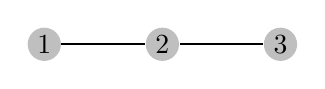
\begin{tikzpicture}[scale=1.5]
    % Draw a 7,11 network
    % First we draw the vertices
    \foreach \pos/\name in {{(1,0)/1}, {(2,0)/2}, {(3,0)/3}}
        \node[vertex] (\name) at \pos {$\name$};
    % Connect vertices with edges 
    \foreach \source/ \dest in {1/2, 2/3}
        \path[edge] (\source) -- (\dest) ;
        
\end{tikzpicture}
\end{center}

They play the repeated $k$-threshold game with $k=3$. Note that after nature moves, player 2 can observe the true state of nature $\theta$, while player 1 or 3 are not. Player 2 plays the role as a coordinator. We can construct an equilibrium which is APEX as the followings. 

\begin{itemize}
\item After nature moves, Rebel 2 chooses $\textbf{revolt}$ if he observes $\theta=(Rebel,Rebel,Rebel)$, and plays \textbf{revolt} in this period. Otherwise, he chooses \textbf{stay} and keeps playing \textbf{stay} afterwards. 
\item After nature moves, Rebel 1 and Rebel 3 play \textbf{stay}.
\item If Rebel 2 chooses \textbf{revolt} in the last period, then Rebel 1 (or Rebel 3) plays \textbf{revolt} in this period; if Rebel 2 chooses \textbf{stay} in the last period, then Rebel 1 (or Rebel 3) keeps playing \textbf{stay} afterwards. 
\item If a Rebel deviates from the above strategy, he will play \textbf{stay} forever; if a Rebel detects a deviation,he will play \textbf{stay} forever.
\end{itemize}

It is straightforward to check that the above strategies constitute an equilibrium if $\delta\geq \frac{1}{2}$. In the equilibrium path, Rebel 1 and Rebel 3 believe that $\{\theta:\#[Rebels](\theta)\geq 3\}$ with probability one if they observe that Rebel 2 has played \textbf{revolt} and believe $\{\theta:\#[Rebels](\theta)< 3\}$ with probability one if Rebel 2 has played \textbf{stay}. Outside of equilibrium path, Rebels arbitrary form their beliefs.
\end{example}



\subsection*{}
I begin to find an APEX equilibrium in general cases.

\section{Equilibrium}
\label{sec:equilibrium}
\subsection{The case: $k=n$}

In Example~\ref{ex_leading_ex}, the construction of an APEX equilibrium relies on some important features. First, since $k=n$, Rebel 2 will never play \textbf{revolt} if one of his neighbor is Inert. Thus, when Rebel 2 plays \textbf{revolt}, it must be the case that all Rebel 2's neighbor are Rebels.  Second, Rebel 1 or Rebel 3 can force Rebel 2 to play \textbf{revolt} to reveal the true state in the first period since only Rebel 2 knows the true state and Rebel 2's actions can separate the states. Third, since $k=n$, one Rebel's shifting to play \textbf{stay} forever is enough to punish a deviation, and so that the group punishment is not necessary. For instance, if a Rebel did not play \textbf{revolt} in the first period at the state $\theta=(Rebel,Rebel,Rebel)$, his neighbor can punish him by playing \textbf{stay} forever. This punishment is credible by letting that player who deviates also plays \textbf{stay} forever. 

I state my result for $k=n$ case as follows.

\begin{theorem}
\label{prop:not_crowded}
For any $n$-person repeated $k$-Threshold game with parameter $k=n$ played in a network, then there is a $\delta^{*}$ such that a sequential APEX equilibrium exists whenever $\delta>
\delta^{*}$.
\end{theorem}
\begin{proof}
Let a strategy profile, $\tau^{*}$, as follows. After nature moves, a Rebel plays \textbf{revolt} if he has no Inert neighbor; a Rebel plays \textbf{stay} forever if he has an Inert neighbor. After first period, if a Rebel has not detected a deviation, and if such Rebel observes that his Rebel neighbors play \textbf{revolt} continuously in the last periods, he keeps playing \textbf{revolt} in the current period; otherwise, he plays \textbf{stay} forever. If a Rebel deviates, then he play \textbf{stay} forever.

According to $\tau^{*}$, at period $s$, if a Rebel has not detected a deviation and if such Rebel observes his Rebel neighbors have played \textbf{stay} once in the last periods, he forms belief $\sum_{\theta:\#[Rebels](\theta)\geq k}\beta^{\pi,\tau^*}_{G_i}(\theta|h^{s}_{G_i})=0$ after period $s$, and therefore playing \textbf{stay} after period $s$ is his best response. If a Rebel detects a deviation or he has deviated to play \textbf{stay}, playing \textbf{stay} is the best response since at least one Rebel will play \textbf{stay}. 

Since the network is finite, if all players do not deviate, there is a finite time $t^{s}_{\theta}$ such that all Rebels play \textbf{revolt} forever if $\theta\in \{\theta: \#[Rebels](\theta)\geq k\}$; and there is a finite time $t^f_{\theta}$ such that all Rebels play \textbf{stay} forever if $\theta\in \{\theta: \#[Rebels](\theta)< k\}$. After $\max\{t^{s}_{\theta},t^f_{\theta}\}$, a Rebel who deviates at most get 0. However, if all Rebels do not deviate, all Rebels get $\max\{1,0\}$ after $\max\{t^{s}_{\theta},t^f_{\theta}\}$. Then, given a period $s>0$, a Rebel will not deviate if $\sum_{\theta:\#[Rebels](\theta)\geq k}\beta^{\pi,\tau^*}_{G_i}(\theta|h^{s}_{G_i})>0$. This because, otherwise, he has a loss in his expected continuation payoff as $\delta^{t^s_{\theta}}\frac{\sum_{\theta:\#[Rebels](\theta)\geq k}\beta^{\pi,\tau^*}_{G_i}(\theta|h^{s}_{G_i})}{1-\delta}$ after $t^s_{\theta}$. There is a $0<\delta<1$ to let such loss be large enough to impede Rebels deviations.

To check if $\tau^{*}$ and $\{\beta^{\pi,\tau^*}_{G_i}(\theta|h^{s}_{G_i})\}_{i\in N}$ satisfy full consistency\footnote{Krep and Wilson (1982)}, take any $0<\eta<1$ such that Rebels play $\tau^{*}$ with probability $1-\eta$, and play other behavior strategies with probability $\eta$. Clearly, when $\eta \rightarrow 0$, the belief converges to $\{\beta^{\pi,\tau^*}_{G_i}(\theta|h^{s}_{G_i})\}_{i\in N}$.
\end{proof}

\begin{remark}
Note that the first best cannot be attained in the equilibrium unless the network is complete. Consider the network in Example~\ref{ex_leading_ex}. Player 1's strategy is not contingent with the true state, and therefore players' actions in the first period are not ex-post efficient.   
\end{remark}





\subsection{The cases : $1<k<n$}

When $k<n$, the equilibrium construction for the $k=n$ case will not work. First, a Rebel still has incentive to play \textbf{revolt} even if there is an Inert neighbor. Second, an Inert never transmit additional information about relevant information since he has only one action. We then require more assumptions to get an APEX equilibrium. Example ~\ref{ex_strong_connectedness} shows why we need additional assumptions.

\begin{example}\label{ex_strong_connectedness}
Let $k=2$ and let the network as the following. Assume $\theta=(Rebel_1,Inert_2,Rebel_3)$.

\begin{center}
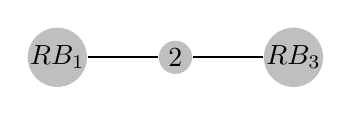
\begin{tikzpicture}[scale=1.5]
    % Draw a 7,11 network
    % First we draw the vertices
    \foreach \pos/\name in {{(1,0)/RB_1}, {(2,0)/2}, {(3,0)/RB_3}}
        \node[vertex] (\name) at \pos {$\name$};
    % Connect vertices with edges 
    \foreach \source/ \dest in {RB_1/2, 2/RB_3}
        \path[edge] (\source) -- (\dest) ;
        
\end{tikzpicture}
\end{center}

First, since $k=2$, Rebel 1 has incentive to play \textbf{revolt} when $\pi(\{\theta:\theta_3=Rebel\})$ is high enough if Rebel 3 will play revolt . Second, Rebel 1 never learn $\theta_3$ since Inert 2 cannot reveal information about $\theta_3$. Thus, the game is reduced to an incomplete information game without communication. Clearly, an APEX equilibrium does not exist in this case.

\end{example}

In order to get an APEX equilibrium and to avoid the case of Example~\ref{ex_strong_connectedness}, I define \textit{Strong connectedness} and \textit{Full support on strong connectedness} as follows.

\begin{definition}
\textbf{Strong connectedness}: Given $G$, a state $\theta$ has strong connectedness if and only if for every pair of Rebels, there is a path consisting of Rebels to connect them.
\end{definition}  

\begin{definition}
\textbf{Full support on strong connectedness}: Given $G$, $\pi$ has full support on strong connectedness if and only if 
\[\pi(\theta)>0\Leftrightarrow \text{ $\theta$ has strong connectedness }\] 
\end{definition}  


The goal of this paper is to show that an APEX equilibrium always exists in the $k<n$ cases when the underlying network is without cycle. I define acyclic network in the following definition.
\begin{definition}
A network is without (with) cycles if and only if the path from $i$ to $j$, for all $i\neq j$, is (is not) unique. 
\end{definition}

I then state my main theorem as follows. 

\begin{theorem}
\label{thm_main_result}
For any $n$-person repeated $k$-Threshold game with parameter $k < n$ played in acyclic networks, if $\pi$ has full support on strong connectedness, then there is a $\delta^{*}$ such that an APEX equilibrium exists whenever $\delta>\delta^{*}$.
\end{theorem}

\subsection*{}
The equilibrium in Theorem ~\ref{thm_main_result} is constructive. I will construct the equilibrium path first, then construct the in-path and off-path beliefs, and then check whether or not there is a strategy profile extending equilibrium path to let the belief system be consistent to constitute an equilibrium. I begin with an overview of equilibrium construction, and then illustrate such construction. The whole equilibrium and the omitted proofs are in the Appendix.  

\subsubsection{Overview}

Given that the state has strong connectedness, Rebels have to find a ``language'' for communication. The construction of an APEX equilibrium is not trivial because the ``dimension'' of information is generally larger than the cardinality of their own action space. Rebels then use several sequences of actions to transmit information, and thus we have to track the belief updating in the time horizontal line and to check whether or not such sequences can constitute an equilibrium. To see that Rebels need to communicate with more dimensions of information, we may compare Example~\ref{ex_cycle_number_5} and Example~\ref{ex_cycle_number_6}.


\begin{example}\label{ex_cycle_number_5}
Let $k=5$ and let the network and the state $\theta$ be the following.

\begin{center} 
  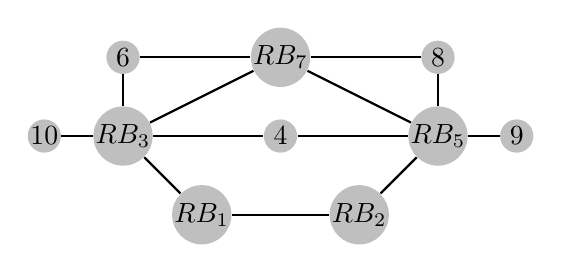
\begin{tikzpicture}[scale=1]
    % First we draw the vertices
    \foreach \pos/\name in {{(2,1)/RB_1}, {(4,1)/RB_2}, {(1,2)/RB_3}, {(5,2)/RB_5}, {(3,3)/RB_7}, {(3,2)/4}, {(1,3)/6}, {(5,3)/8}, {(6,2)/9}, {(0,2)/10}}
        \node[vertex] (\name) at \pos {$\name$};
        
%        \foreach \pos/\name in {{(3,2)/4_L}, {(1,3)/6_L}, {(5,3)/8_L}, {(6,2)/9_L}, {(0,2)/10_L}}
%   \node[selected vertex] (\name) at \pos {$\name$};
    
    % Connect vertices with edges 
    \foreach \source/ \dest in {RB_1/RB_2, RB_1/RB_3, RB_2/RB_5, RB_3/4, RB_3/6, RB_3/RB_7, 4/RB_5, RB_5/RB_7, RB_5/8, RB_5/9,6/RB_7, RB_7/8, RB_3/10}
        \path[edge] (\source) -- (\dest) ;
\end{tikzpicture}
\end{center} 

\end{example}


\begin{example}\label{ex_cycle_number_6}
Let $k=6$ and let the network and the state $\theta$ be the following.
\begin{center} 
  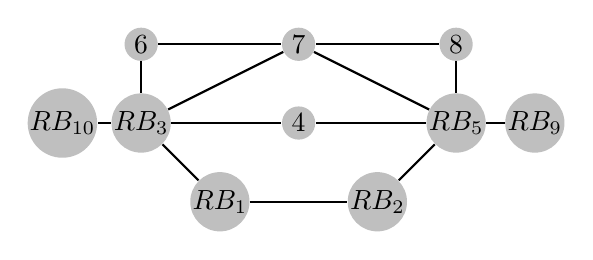
\begin{tikzpicture}[scale=1]
    % First we draw the vertices
    \foreach \pos/\name in {{(2,1)/RB_1}, {(4,1)/RB_2}, {(1,2)/RB_3}, {(5,2)/RB_5}, {(3,3)/7}, {(3,2)/4}, {(1,3)/6}, {(5,3)/8}, {(6,2)/RB_9}, {(0,2)/RB_{10}}}
        \node[vertex] (\name) at \pos {$\name$};
        
%        \foreach \pos/\name in {{(3,2)/4_L}, {(1,3)/6_L}, {(5,3)/8_L}, {(6,2)/9_L}, {(0,2)/10_L}}
%   \node[selected vertex] (\name) at \pos {$\name$};
    
    % Connect vertices with edges 
    \foreach \source/ \dest in {RB_1/RB_2, RB_1/RB_3, RB_2/RB_5, RB_3/4, RB_3/6, RB_3/7, 4/RB_5, RB_5/7, RB_5/8, RB_5/RB_9,6/7, 7/8, RB_3/RB_{10}}
        \path[edge] (\source) -- (\dest) ;
\end{tikzpicture}
\end{center} 


\end{example}

In Example~\ref{ex_cycle_number_6}, there are 6 Rebels. On the contrary, there are 5 Rebels in Example~\ref{ex_cycle_number_5}. Suppose that we have a ``talking strategy'' as follows. Rebel 3 and Rebel 5 report the numbers of  Rebels in their neighborhood to Rebel 1 and Rebel 2. Rebel 1 and Rebel 2 then talk with each other about the total number of Rebels they have been informed conditional on Rebel 3 and Rebel 5's reporting. Conditional on the total number of Rebels they have been informed, Rebel 1 and Rebel 2 then initiate the coordination to play revolt or to play revolt. According to this talking strategy, however, Rebel 1 and Rebel 2 still do not know how many Rebels out there. This is because Rebel 3 and Rebel 5 report the same number of Rebel neighbors in both Example~\ref{ex_cycle_number_6} and Example~\ref{ex_cycle_number_5}. Thus, ``talking about how many nearby Rebels"  is not enough, Rebels have to ``talking about the locations of nearby Rebels''  in order to construct an APEX strategy. 

Moreover, in an APEX equilibrium path, \text{all} Rebels must tell whether or not there are more than $k$ Rebels in the equilibrium path at some timings. To see this, I give the following lemma.
\begin{lemma}\label{lemma_learn}
Given $G$, $\pi$, $\delta$, $k$. If a weak sequential equilibrium $\tau^*$ is APEX, then for all $\theta\in \Theta$, there is a finite time $T^{\theta}_i$ for a Rebel $i$ such that $\sum_{\theta:\#[Rebels](\theta)\geq k}\beta^{\pi,\tau^*}_{G_i}(\theta|h^{s}_{G_i})$ either $=1$ or $=0$
whenever $s\geq T^{\theta}_i$.
\end{lemma}
The question is how to track each Rebel's timing in which he has known the relevant information. This higher-order belief is apparently an giant object in our private monitoring setting. To overcome the difficulty in tracking each Rebel's learning process, I let Rebels use several ``coordination sequences'' to communicate with others when they have known that some Rebels (including themselves) have known the relevant information.


In my construction, the off-path belief system gives the grim-trigger property. To be more precise, if a Rebel $i$ detects a deviation at period $s$, his off-path belief will be $\sum_{\theta \in \{\theta:\theta_j=Inert,j\notin G_i\}}\beta^{\pi,\tau}_{G_i}({\theta}|h^{s^{'}}_{G_i})=1$ for all $s^{'}\geq s$. I.e., he will believe that all players outside his neighborhood are Inerts, and therefore he will stop update his belief about relevant information. The consequence is that he will play \textbf{stay} forever if there are less than $k$ Rebel neighbors in his neighborhood. 

The equilibrium is constructed by three steps. I list these three steps in the following consecutive three subsections. In the first step, I define the \textit{information hierarchy} to specify which Rebels in $G$ have to report their information in the equilibrium path. In the second step, I construct the equilibrium path by using binary-$\{\textbf{revolt},\textbf{stay}\}$ sequences, and check the belief updating in the path. Finally, I use the grim-trigger-like off-path belief as a punishment schema to impede deviations in the third step.  

\subsubsection{Step 1. Information hierarchy in $G$}

The information hierarchy is defined on a network $G$ right after nature chooses a state. I will use the term ``node $i$'' instead of ``player $i$'' in this step. 

I define information hierarchy by defining $\{N^{-1}_i,N^{0}_i, N^{1}_i...\}$ and $\{I^{-1}_i,I^{0}_i, I^{1}_i...\}$ for each $i\in N$, and then define $\{\leq^0, \leq^1, \leq^2\}$ and $\{R^0,R^{1}, R^{2}...\}$ for each iteration in $(0,1,2,...)$. I also use the term ``blocks'' to represent the ``iterations''. 

Given $\theta$, the information hierarchy is defined as follows.
\begin{itemize}

\item \textbf{0-block}
Denote
\begin{eqnarray*}
N^{-1}_i &\equiv &  i \\
I^{-1}_i & \equiv & i
\end{eqnarray*}

Then define $R^0$ as 
\begin{equation}
R^0\equiv [Rebels](\theta)
\end{equation}

\item \textbf{1-block}
Denote
\begin{eqnarray*}
N^0_i &\equiv &  G_i \\
I^0_i & \equiv & G_i\cap R^0
\end{eqnarray*}

Define the set $\leq^0$ by defining
\begin{equation}i\in \leq^0 \Leftrightarrow \exists  j\in \bar{G}_i [I^0_i\subseteq N^0_j\cap R^0]\end{equation}  

Then define $R^1$ as 
\begin{equation}
R^{1} \equiv \{i\in R^0|i\notin \leq^0\}
\end{equation}

\item \textbf{$t+1$-block, $t\geq 1$}
Denote
\begin{eqnarray*}
N^t_i & \equiv & \bigcup_{k\in I^{t-1}_i}G_k \\
I^t_i & \equiv & \bigcup_{k\in G_i\cap R^t}I^{t-1}_k
\end{eqnarray*}


Define the set $\leq^t$ by defining
\begin{equation}i\in \leq^t \Leftrightarrow \exists j\in \bar{G}_i[I^t_i\subseteq N^t_j\cap R^0]\end{equation}

Then define $R^{t+1}$ as 
\begin{equation}
R^{t+1} \equiv  \{i\in R^t|i\notin \leq^t\}
\end{equation}


\end{itemize}

In other words, $i\in R^t$ if and only if \textit{(1)} $i$ is a Rebel and \textit{(2)} at $t$-block, there is a $j\in I^{t-1}_i$ who is a Rebel and whose existence is informed to $i$, but none of $i$'s neighbors has been informed that. Intuitively, the $R^t$ nodes then have more incentives to report their information to others. 

From the above definition, Theorem ~\ref{lemma_empty} states that it is sufficient to only let $R^t$ nodes to report their information if the underlying network is acyclic. 
\begin{theorem}
\label{lemma_empty}
If the network is acyclic and if the state has strong connectedness, then 
\[R^0\neq \emptyset \Rightarrow \exists t\geq 0[\exists i\in R^t[I^t_i=R^0]]\]
\end{theorem}



\subsubsection{Step 2: Equilibrium strategies in the path}


In this step, I first assigned each player in $G$ a distinguished prime number to indicate his ``location''. Such indexation is starting from $3$. To be more precise, I index each player $i$ as $x_i$, where $x_i\geq 3$ is a prime number. Since the multiplication of distinguish prime numbers can be uniquely factorized as those numbers, I then use this property to let Rebels be able to report both the amount and the locations of their Rebel neighbors by reporting the multiplication of their Rebel neighbors' prime numbers.

Denote $\langle\rangle$ as a form of sequence. Denote $|\langle\rangle|$ as the length of a form of finite sequence. Denote $\bar{N}\subset N$ as an non-empty subset of $N$. The notations for the forms of sequences are shown in Table ~\ref{Table_msg_form}. 

\begin{table}[t]
\caption{Notations}
\label{Table_msg_form}
\begin{center}
\begin{tabular}{l c c}
$\bar{N}$ 										& $\equiv$ 			& a non-empty subset of $N$  \\
$x_i$ 											& $\equiv$ 			& player $i$'s prime-number index  \\
$X_{\bar{N}}$ 								& $\equiv$ 			& $\prod_{j\in \bar{N}}x_j$  \\
\textbf{s}										& $\equiv$ 			& \textbf{stay}  \\
\textbf{r}										& $\equiv$ 			& \textbf{revolt}  \\
$\langle \textbf{stay} \rangle$ 		& $\equiv$ 			& $\langle \textbf{s},...,\textbf{s}\rangle$  \\
$\langle \textbf{revolt} \rangle$ 	& $\equiv$ 			& $\langle \textbf{r},...,\textbf{r}\rangle$  \\
$\langle  \bar{N} \rangle$ 				& $\equiv$ 			& $\langle \textbf{s},...,\textbf{s},\underbrace{\textbf{r},\textbf{s},...,\textbf{s}}_{X_{ \bar{N}}}\rangle$  \\

$\langle 1 \rangle$	 					& $\equiv$ 			& $\langle \textbf{s},...,\textbf{s},\underbrace{\textbf{r}}_{1}\rangle$  \\
$\langle x_i \rangle$	 	& $\equiv$ 			& $\langle \textbf{s},...,\textbf{s},\underbrace{\textbf{r},\textbf{s},...,\textbf{s}}_{x_i}\rangle$  \\
\end{tabular}
\end{center}
\end{table}

The $\langle\rangle$ and the $|\langle\rangle|$ will jointly determine the sequences of actions in the equilibrium path. For example, if a sequence takes the form $\langle 1 \rangle$ and its length $|\langle 1 \rangle|=3$, then this sequence is $\langle \textbf{s},\textbf{s},\textbf{r}\rangle$. Note that the length of a sequence is counted from its end.



In the equilibrium path, two phases, \textit{reporting period} and \textit{coordination period}, occur in turns finitely in the following way,
\[\underbrace{<\text{coordination period}>}_{0-block}\underbrace{<\text{reporting period}><\text{coordination period}>}_{1-block}...\]
I.e. after nature chooses a state, all the Rebels start with $0$-block, then enter to $1$-block,...,and so on. $0$-block has only one period, coordination period. The $t$-blocks, $t\geq 1$ has two periods, reporting period and coordination period, where reporting period occurs first and then coordination period follows. The length of each phase in each block is finite but endogenous.

If a sequence of actions is meant to be played in the reporting period (\textit{resp.} the coordination period), I called it a \textit{reporting message} (\textit{resp.} \textit{coordination message}). In reporting period in each $t$-block ($t\geq 1$), Rebels play the sequences defined in Table ~\ref{Table_msg_reporting}. In coordination period in each $t$-block ($t\geq 0$), Rebels play the sequences defined in Table ~\ref{Table_msg_coordination}. After the coordination period in each $t$-block ($t\geq 0$), players either \textit{(1)} start to repeatedly play some certain actions,  or \textit{(2)} enter to the reporting period in $t+1$-block. 


\subsubsection*{}
I start to give the details of reporting messages and coordination messages.


\subsubsection*{Reporting messages in reporting period}

Denote $|\langle RP^t \rangle|$ be the total number of periods in the $t$-block reporting period. In the equilibrium path, the sequence played in the $t$-block reporting period has to be in one kind of forms listed 
Table ~\ref{Table_msg_reporting}. Any sequence played differently will be considered as a deviation. 

\begin{table}[ht]
\caption{Reporting messages}
\label{Table_msg_reporting}
\begin{center}
\begin{tabular}{c c }
Reporting Messages 		&   \\
\hline
$\langle  \textbf{stay} \rangle$ 	& 	 \\
$\langle  {I^{t-1}_i} \rangle$ 		&   \\
$\langle 1 \rangle$ 		             &    
\end{tabular}
\end{center}
\end{table}

Table ~\ref{Table_blf_up_reporting} shows that the belief formed by Rebel $j$ after $j$ observe his neighbor $i$'s reporting messages in the equilibrium path.

\begin{table}[ht]
\caption{$j$'s belief updating after observing $i$'s reporting messages in the reporting period in $t$-block}
\label{Table_blf_up_reporting}
\begin{center}
\begin{tabular}{l c l}
$i$ plays 		&  			& the event that $j\in \bar{G}_i$ believes with probability one  \\
\hline
$\langle  \textbf{stay} \rangle$ 	& 			    & $i\notin R^t$  \\
$\langle  {I^{t-1}_i} \rangle$ 		&  			& $i\in R^t$ and $l\in [Rebel](\theta)$ if $l\in I^{t-1}_i$      \\
$\langle 1 \rangle$ 		             &  			& $i\in R^t$ and $i$ has known $\#[Rebels](\theta)\geq k-1$ \\
\end{tabular}
\end{center}
\end{table}

According to Table ~\ref{Table_blf_up_reporting}, a Rebel can tell who are $R^t$ after reporting period. The consequence is that, if a Rebel $j$ has observed that all of his neighbors are not in $R^t$, then he is sure that $\#[Rebels](\theta)< k$ if $\#I^{t-1}_j<k$\footnote{Remind that $R^t$ are those Rebels who have been informed the existence of some Rebels, but any of their neighbors has not been informed that.}. 


The important feature here is the usage of $\langle 1 \rangle$. It serve as a signal to indicate a pivotal player and to solve free rider problems. I elaborate this issue here by providing some examples. Free rider problems may happen if Rebels' coordination messages do not contingents on their reporting messages in the equilibrium path. We may consider the Example~\ref{ex_free_rider_tree}.

\begin{example} \label{ex_free_rider_tree}\textbf{Free Rider Problem}

Let $k=5$ and assume that there are message $\langle M_4 \rangle,\langle M_5 \rangle$ for Rebel 4, 5. To simply the analysis, let's assume that the game is played from $1$-block (by discarding the strategies in $0$-block and staring the game from the reporting period). Further, assume that Rebels will play \textbf{revolt} forever after observing that $\langle M_4 \rangle$ or $\langle M_5 \rangle$ is played once by Rebel 4 or 5 right after reporting period; otherwise they will play \textbf{stay} forever. Let $G$ be the following.

\begin{center}
\begin{tikzpicture}[scale=1]
    % Draw a 7,11 network
    % First we draw the vertices
    \foreach \pos/\name in {{(1,2)/RB_1}, {(2,1)/RB_2}, {(2,3)/3}, {(3,2)/RB_4}, {(4,2)/RB_5}, {(5,1)/6}, {(5,3)/7}, {(6,2)/RB_8}}
        \node[vertex] (\name) at \pos {$\name$};
    
    
    % Connect vertices with edges 
    \foreach \source/ \dest in {RB_1/4, RB_2/RB_4,3/RB_4,RB_4/RB_5, RB_5/6, RB_5/7, RB_5/RB_8}
        \path[edge] (\source) -- (\dest) ;
        
\end{tikzpicture}
\end{center}

Note that Rebel 4 and Rebel 5 are $R^1$ members. Let $\langle \rangle_4$ and $\langle \rangle_5$ be the sequences of actions they may use to report the number of Rebel neighbors. If Rebel 5 report truthfully, then Rebel 4 will not report truthfully by arranging the timings in which he plays \textbf{revolt}. Since Rebel 4 can use $\langle M_4 \rangle$ to initialize the coordination, such deviation is profitable. Same situation happens for Rebel 5, and then Rebel 4 and Rebel 5 will not report truthfully.

\end{example}

In the above example, two sources constitutes the free rider problem. One source is that there is a coordination message which will initiate coordination regardless how the reporting messages are played. The other source is that Rebel 4 and Rebel 5 are \textit{pivotal}---they are certain that they will learn the true state given others' truthful reporting  right after reporting period. To see the later source more clearly, we may consider the following Example~\ref{ex_pivotal_1}.



\begin{example} \label{ex_pivotal_1}\textbf{Pivotal player: Case 1}
Let $k=6$ and suppose that there are message $\langle M_3 \rangle,\langle M_5 \rangle, \langle M_7 \rangle$ for Rebel 3,5,7 to initiate a coordination. Let the game be played from $1$-block as Example~\ref{ex_free_rider_tree}. Further, let's suppose that Rebels will play \textbf{revolt} forever after observing that $\langle M_3 \rangle$, $\langle M_5 \rangle$, or $\langle M_7 \rangle$ is played once in two periods right after this reporting period; otherwise they will play \textbf{stay} forever. Let $G$ be the following.
\begin{center}
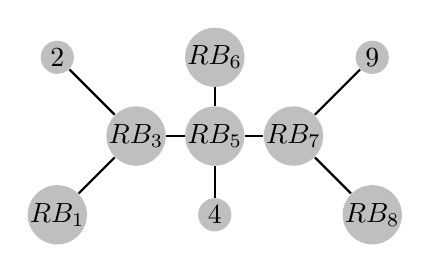
\begin{tikzpicture}[scale=1]
    % Draw a 7,11 network
    % First we draw the vertices
    \foreach \pos/\name in {{(1,1)/RB_1}, {(1,3)/2}, {(2,2)/RB_3}, {(3,1)/4}, {(3,2)/RB_5}, {(3,3)/RB_6}, {(4,2)/RB_7}, {(5,1)/RB_8}, {(5,3)/9}}
        \node[vertex] (\name) at \pos {$\name$};
    
    
    % Connect vertices with edges 
    \foreach \source/ \dest in {RB_1/RB_3, 2/RB_3,RB_3/RB_5,4/RB_5, RB_6/RB_5, RB_5/RB_7, RB_7/RB_8, RB_7/9}
        \path[edge] (\source) -- (\dest) ;
        
\end{tikzpicture}
\end{center}

Note that Rebel 3, 5, 7 are $R^1$ members. In contrast to Example~\ref{ex_free_rider_tree}, although Rebel 3, 7 can use their coordination messages to initiate coordination, they still have incentives to report truthfully. This is because they can not know the true state right after the reporting period. Then, since the coordination to \textbf{revolt} has to be initiated immediately after this reporting period, they have incentives to report truthfully to Rebel 5.

Rebel 5, however, has no incentive to report truthfully since he is certain that he will know the true state immediately after the reporting period.
\end{example}
   
From the discussions in Example~\ref{ex_free_rider_tree} and Example~\ref{ex_pivotal_1}, a way to deal with the free rider problem is to identify who are the pivotal players in each reporting period. If we can identify them, we can let them report nothing but sending the coordination messages. If the networks are FFCCU without cycles, Lemma ~\ref{lemma_at_most_two_nodes} shows that the free rider problem can be identified before the game enter to $t$-block and the pivotal player can be identified either. More precisely, first define $Tr_{ij}$ as a tree rooted in $i$ node while it leaves spanning from $j\in \bar{G}_i$.

\begin{definition}
$Tr_{ij}\equiv \{l\in N:\text{there is a unique path $\{l,...,j,i\}$ from $l$ to $i$ through $j$}\}$
\end{definition}
and define the set
\[C^t=\{i\in R^t:\nexists j\in R^{t-1}\cap \bar{G}_i[\exists l,l^{'}\in Tr_{ij}[l\in N^{t-1}_j\backslash I^{t-1}_i \text{ and } l^{'}\in \bar{G}_l]]\}\]
be those $R^t$ nodes such that there are no possible Rebel nodes connect with them by a path in which there are more than three nodes. For instance, the nodes Rebel 4 and Rebel 5 in Example~\ref{ex_free_rider_tree} are $C^1$ nodes and Rebel 5 in Example~\ref{ex_pivotal_1} is also a $C^1$ node. Then we can show the following lemmas. 

\begin{lemma}
\label{lemma_at_most_two_nodes}
If the network is FFCCU without cycle, and  if the state has strong connectedness, then for each $t$-block
\begin{enumerate}
\item $0\leq |C^t| \leq 2$.
\item Moreover, suppose there are two nodes in $C^t$, then they are each other's neighbor.
\end{enumerate}
\end{lemma}


\begin{lemma}
\label{lemma_no_node_outside}
If the network is FFCCU without cycle, and if the state has strong connectedness, then for each $t$-block
\[i\in C^t \Rightarrow \text{there is no possible Rebel node outside of }\bigcup_{k\in N^{t-1}_i}G_k\]
\end{lemma}

Lemma ~\ref{lemma_at_most_two_nodes} is crucial because $C^t$-nodes can identify each other by the following procedure. First, a $C^t$-node ,$j$, assume that one of his $R^{t-1}$ neighbor, $i$, is a $R^t$-node. Second, he check if $i$ is in $C^t$ by checking the definition of $C^t$. Third, if $i$ is identified as a $C^t$ node, $i$ is the only other candidate. Finally, he assume that $i$ will do the same procedure to identify him. Since himself is a $C^t$-node, $i$ must be able to identify him if $i$ is a $C^t$-node, and thus both $C^t$-nodes can identify each other.

If there are more than one $C^t$ nodes, I pick a node who has smaller prime index to be a pivotal player\footnote{This property is not generally hold if a network has cycle.}. Lemma ~\ref{lemma_no_node_outside} characterize the intuition behind Example~\ref{ex_free_rider_tree} and~\ref{ex_pivotal_1}.

However, Lemma ~\ref{lemma_no_node_outside} does not show only the node in $C^t$ are pivotal. Some pivotal players thus can not be identified before the game enter $t$-block. Since that, we have to identify them during the game is played, and therefore we have to track their evolving information sets sequentially. This another source to let players become pivotal is that \textit{a Rebel has already known too much}, and therefore he is sure that he will learn {either $\#[Rebels](\theta)\geq k$ or $\#[Rebels](\theta)< k$} after current reporting period. Example~\ref{ex_pivotal_2} give a concrete example.

\begin{example} \label{ex_pivotal_2}\textbf{Pivotal player: Case 2}
Let $k=6$. Again, assume that there are coordination message $\langle M\rangle$s for Rebels. Let the game play starting from $1$-block as Example~\ref{ex_free_rider_tree}. Again, assume Rebel will play \textbf{revolt} forever after observing $\langle M \rangle$ being played once in four periods\footnote{It requires four periods to let the coordination message transmit.} immediately after reporting period; otherwise they will play \textbf{stay} forever. Let $G$ be the followings.

\begin{center}
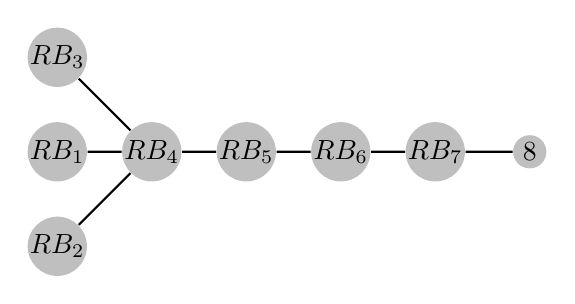
\begin{tikzpicture}[scale=1.2]
    % Draw a 7,11 network
    % First we draw the vertices
    \foreach \pos/\name in {{(2,2)/RB_1}, {(2,1)/RB_2}, {(2,3)/RB_3}, {(3,2)/RB_4}, {(4,2)/RB_5}, {(5,2)/RB_6}, {(6,2)/RB_7}, {(7,2)/8}}
        \node[vertex] (\name) at \pos {$\name$};
    
    
    % Connect vertices with edges 
    \foreach \source/ \dest in {RB_1/RB_4, RB_2/RB_4,RB_3/RB_4,RB_4/RB_5, RB_5/RB_6, RB_6/RB_7, RB_7/8}
        \path[edge] (\source) -- (\dest) ;
        
\end{tikzpicture}
\end{center}

In this case, no Rebels are in $C^1$, but Rebel 4 will deviate from reporting $\langle I^0_4 \rangle$. Note that Rebel 4 has already known there are 5 Rebels in this world, therefore knowing one more Rebels is enough to initiate the coordination to \textbf{revolt}. Moreover, if there is no more Rebels, the only coordination is the coordination to \textbf{stay}. If node 6 is a Rebel, Rebel 5 will report that, and therefore he will know $\#[Rebels](\theta)\geq 6$; Otherwise, due to the state has strong connectedness, he will also know $\#[Rebels](\theta)< 6$ for sure immediately after reporting period. Since he can use the message $\langle M \rangle$ to initiate the coordination, this deviation is profitable.
\end{example}

After the discussion in the above examples, the message $\langle 1 \rangle$ is introduced to specify the pivotal players. In the equilibrium path in the Appendix, the pivotal players in $t$-block are those Rebels who have already known there are $k-1$ Rebels before they report their $I^{t-1}$ in the equilibrium path, or who are in $C^t$. The pivotal players will play $\langle 1 \rangle$ in the equilibrium path, and therefore the beliefs after observing $\langle 1 \rangle$ is that \textit{a Rebel has known $\#[Rebels](\theta)\geq k-1$} in the the path as Table ~\ref{Table_blf_up_reporting} shows.




\subsubsection*{Coordination messages in coordination period}

The ignorance of reporting messages after observed a coordination message $\langle M \rangle$ may incur untruthfully reporting as the above Example~\ref{ex_free_rider_tree}, ~\ref{ex_pivotal_1}, and ~\ref{ex_pivotal_2} show, and the introducing of messages $\langle 1 \rangle$ is meant to tackle with this issue. However, one may have observed that the combination of these two messages, $\langle 1 \rangle\langle M \rangle$, themselves is another ``coordination message''. I.e., $\langle\langle \textbf{s}, \textbf{r} \rangle\langle M \rangle\rangle$ is another coordination message by truncating previous actions of $\langle 1 \rangle$ and concatenate the remaining to $\langle M \rangle$. If the contingent behavior after observing this new coordination message is the same as seeing the original one, $\langle M \rangle$, the untruthfully reporting problem has not been solved. In this section, I still let $\langle 1 \rangle$ as a reporting messages and call those $\langle M \rangle$ coordination messages, but I let the belief updating be contingent not only on the coordination messages but also on reporting messages.


There are three divisions in coordination period and there are several sub-blocks in each division. In $t=0$ block, the form is
\[\overbrace{\langle\underbrace{\langle \cdot \rangle }_{\text{$1$ sub-block}}\rangle}^{\text{1st division}} \overbrace{\langle\underbrace{\langle \cdot \rangle }_{\text{$1$ sub-blocks}} \rangle}^{\text{2nd division}} \overbrace{\langle\underbrace{\langle \cdot \rangle \cdot \cdot \cdot \langle \cdot \rangle}_{\text{$n$ sub-blocks}}\rangle}^{\text{3rd division}}\] 
; in $t>0$ blocks, the form is
\[\overbrace{\langle\underbrace{\langle \cdot \rangle \cdot \cdot \cdot \langle \cdot \rangle}_{\text{$n$ sub-blocks}}\rangle}^{\text{1st division}} \overbrace{\langle\underbrace{\langle \cdot \rangle \cdot \cdot \cdot \langle \cdot \rangle}_{\text{$t+1$ sub-blocks}} \rangle}^{\text{2nd division}} \overbrace{\langle\underbrace{\langle \cdot \rangle \cdot \cdot \cdot \langle \cdot \rangle}_{\text{$n$ sub-blocks}}\rangle}^{3rd division}\] 
, where $n=\# N$. 


Denote $CD^t_{m,q}$ be the $m$ sub-block in $q$ division, and denote $|\langle CD^t_{m,q} \rangle|$ be the total number of periods in $CD^t_{m,q}$.  The outcome of pure strategies in equilibrium path takes the following forms of sequences with length $|\langle CD^t_{m,q} \rangle|$ as Table ~\ref{Table_msg_coordination} shows.
\begin{table}[ht]
\caption{Coordination messages}
\label{Table_msg_coordination}
\begin{center}

\begin{tabular}{cc }
Coordination messages		&   \\
\hline
$\langle x_i \rangle$ 	& 	 \\
$\langle \textbf{stay} \rangle$	&   \\
\textbf{r}									& 	\\
\textbf{s}									& 	\\
\end{tabular}
\end{center}
\end{table}

If there is a Rebel who has at least $k$ Rebels neighbors, all the Rebels will play \textbf{revolt} after $0$-block in the equilibrium path. Since $0$-block has simpler structure, I will focus on the behaviors in the coordination period in $t>0$ block in the following paragraphs, while the Appendix shows the equilibrium path in $t=0$ block. 

The belief a Rebel $j$ form after observing $i$ after $CD^t_{1,1}$ in equilibrium path is as Table ~\ref{Table_blf_up_cdt11} shows. After $CD^t_{1,1}$, Rebel $j$ will be notified one more event: $\#[Rebels](\theta)< k$. Clearly, $j$ will play \textbf{stay} forever if this event has been notified. In order to transmit this information about this event, Rebels will play $\langle x_i \rangle$ unless they observe someone play $\langle \textbf{stay} \rangle$ in the path in $CD^t_{m,1}$ where $m\geq 2$ as Table ~\ref{Table_stg_cdt21} and Table ~\ref{Table_stg_cdtm1} shows. After $CD^t_{n,1}$, the information of $\#[Rebels](\theta)< k$ will be transmitted across all players. 
\begin{table}[ht]
\caption{Belief updating after $CD^t_{1,1}$, $t>0$}
\label{Table_blf_up_cdt11}
\begin{center}
\begin{tabular}{c c c}
In $RP^t$ 	&  	In $CD^t_{1,1}$		&  \\
\hline
\hline
$i$ plays 		&  	$i$ plays		& The events $j\in \bar{G}_i$ believe with probability one  \\
\hline
$\langle  \textbf{stay} \rangle$ 	& 	$\langle x_i \rangle$	    & $i\notin R^t$ \\
$\langle  {I^{t-1}_i} \rangle$ 		&  $\langle \textbf{stay} \rangle$		& $\#[Rebels](\theta)< k$     \\
$\langle  {I^{t-1}_i} \rangle$ 		&  $\langle x_i \rangle$		& $i\in R^t$     \\
$\langle 1 \rangle$ 		             &  $\langle \textbf{stay} \rangle$		& $\#[Rebels](\theta)< k$  \\
$\langle 1 \rangle$ 		             &  $\langle x_i \rangle$		&  $\#[Rebels](\theta)\geq k$ 
\end{tabular}
\end{center}
\end{table}



\begin{table}[ht]
\caption{In-path strategies in $RP^t$, $CD^t_{1,1}$, and $CD^t_{2,1}$, $t>0$}
\label{Table_stg_cdt21}
\begin{center}
\begin{tabular}{c c c}
In $RP^t$ 	 	&  	In $CD^t_{1,1}$		&  In $CD^t_{2,1}$	\\
\hline
\hline
$i$ plays 		  							&  	$i$ plays									& $j\in \bar{G}_{i}$ plays  \\
\hline
$\langle  \textbf{stay} \rangle$ 	& 	$\langle x_i \rangle$	    & $\langle x_i \rangle$ \\
$\langle  {I^{t-1}_i} \rangle$ 		&  $\langle \textbf{stay} \rangle$		& $\langle \textbf{stay} \rangle$     \\
$\langle  {I^{t-1}_i} \rangle$ 		&  $\langle x_i \rangle$		& $\langle x_i \rangle$     \\
$\langle 1 \rangle$ 		             &  $\langle \textbf{stay} \rangle$		& $\langle \textbf{stay} \rangle$  \\
$\langle 1 \rangle$ 		             &  $\langle x_i \rangle$		&  $\langle x_i \rangle$  
\end{tabular}
\end{center}
\end{table}

\begin{table}[ht]
\caption{In-path strategies after $CD^t_{m,1}$, where $m\geq 2$, $t>0$}
\label{Table_stg_cdtm1}
\begin{center}
\begin{tabular}{c c c}
In $CD^t_{m,1}$, $m\geq 2$ 	 	&  	In $CD^t_{m+1,1}$,$m\geq 2$		& 	\\
\hline
\hline
$i$ plays 		  							&  $j\in \bar{G}_{i}$ plays  								& \\
\hline
$\langle x_i \rangle$ 	& 	$\langle x_i \rangle$	    &  \\
$\langle \textbf{stay} \rangle$		&  $\langle \textbf{stay} \rangle$	&  \\

\end{tabular}
\end{center}
\end{table}



Game enter to $CD^t_{1,2}$. In $CD^t_{1,2}$, Rebels start to check if the coordination to \textbf{revolt} can be initiated. The coordination message to initiate the coordination is $\langle \textbf{stay} \rangle$ as Table ~\ref{Table_blf_up_cdt12} shows. The important features here is that $\langle \textbf{stay} \rangle$ is a coordination message \textit{only if} $\langle  {I^{t-1}_i} \rangle$ or $\langle 1 \rangle$ has been played in reporting period.  First, note that $\langle \textbf{stay} \rangle$ is also the message to coordinate to \textbf{stay} in $CD^t_{m,1}$, $m\geq 1$ and note that this is the only candidate to be a message to coordinate to \textbf{stay}. Rebels are not confused about the information which \textbf{stay} carries since the information is now contingent on the reporting messages. Second, $\langle \textbf{stay} \rangle$ incurs no expected cost in equilibrium path. It is important because otherwise a free rider problem will happen again if such message incurs expected costs. Third, since this message is contingent on the reporting messages, initiating the coordination to \textbf{revolt} is ``not free'' since it requires Rebels to report something in reporting period to initiate that. This trade-off between reporting something and reporting nothing will force Rebels to report something in reporting period in order to take chances to initiate the coordination to \textbf{revolt}.

After the initiating in $CD^t_{1,2}$, Rebels start to transmit the information of $\#[Rebels](\theta)\geq k$ in $CD^t_{m,2}$ $m\geq 2$ as Table ~\ref{Table_stg_cdt12} and Table ~\ref{Table_stg_cdtm2} shows. That is, they will play $\langle \textbf{stay} \rangle$ unless they observe someone play $\langle x_i \rangle$. After $CD^t_{{t+1},1}$, the information of $\#[Rebels](\theta)\geq k$ will be transmitted across at least $k$ Rebels. 

\begin{table}[ht]
\caption{Belief updating after $CD^t_{1,2}$, $t>0$}
\label{Table_blf_up_cdt12}
\begin{center}
\begin{tabular}{l c c c}
In $RP^t$ 	 	&  	In $CD^t_{1,1}$		&  In $CD^t_{1,2}$	  &\\
\hline
\hline
$i$ plays 		                             &  	$i$ plays		&				$i$ plays			& The events $j$ believe with probability one  \\
\hline
$\langle  \textbf{stay} \rangle$ 	& 	$\langle x_i \rangle$	&  $\langle \textbf{stay} \rangle$ &  $i\notin R^t$ \\
$\langle  {I^{t-1}_i} \rangle$ 		&  $\langle \textbf{stay} \rangle$	&	$\langle \textbf{stay} \rangle$ &  $\#[Rebels](\theta)< k$   \\
$\langle  {I^{t-1}_i} \rangle$ 		&  $\langle x_i \rangle$	&	$\langle \textbf{stay} \rangle$ &  $\#[Rebels](\theta)\geq k$    \\
$\langle  {I^{t-1}_i} \rangle$ 		&  $\langle x_i \rangle$	&	$\langle x_i \rangle$ &  $i\in R^t$  \\
$\langle 1 \rangle$ 		             &  $\langle \textbf{stay} \rangle$	&	$\langle \textbf{stay} \rangle$ &  $\#[Rebels](\theta)< k$\\
$\langle 1 \rangle$ 		             &  $\langle x_i \rangle$	&	$\langle \textbf{stay} \rangle$ & $\#[Rebels](\theta)\geq k$
\end{tabular}
\end{center}
\end{table}




\begin{table}[ht]
\caption{In-path strategies in $RP^t$, $CD^t_{1,1}$, $CD^t_{1,2}$, and $CD^t_{2,2}$, $t>0$}
\label{Table_stg_cdt12}
\begin{center}
\begin{tabular}{l c c c}
In $RP^t$ 	 	&  	In $CD^t_{1,1}$		&  In $CD^t_{1,2}$	  & In $CD^t_{2,2}$ \\
\hline
\hline
$i$ plays 		                             &  	$i$ plays		&				$i$ plays			& $j\in \bar{G}_i$ plays  \\
\hline
$\langle  \textbf{stay} \rangle$ 	& 	$\langle x_i \rangle$	&  $\langle \textbf{stay} \rangle$ &  $\langle \textbf{stay} \rangle$ \\
$\langle  {I^{t-1}_i} \rangle$ 		&  $\langle \textbf{stay} \rangle$	&	$\langle \textbf{stay} \rangle$ &  $\langle \textbf{stay} \rangle$   \\
$\langle  {I^{t-1}_i} \rangle$ 		&  $\langle x_i \rangle$	&	$\langle \textbf{stay} \rangle$ &  $\langle x_i \rangle$    \\
$\langle  {I^{t-1}_i} \rangle$ 		&  $\langle x_i \rangle$	&	$\langle x_i \rangle$ &  $\langle \textbf{stay} \rangle$  \\
$\langle 1 \rangle$ 		             &  $\langle \textbf{stay} \rangle$	&	$\langle \textbf{stay} \rangle$ &  $\langle \textbf{stay} \rangle$\\
$\langle 1 \rangle$ 		             &  $\langle x_i \rangle$	&	$\langle \textbf{stay} \rangle$ & $\langle x_i \rangle$
\end{tabular}
\end{center}
\end{table}

\begin{table}[ht]
\caption{In-path strategies after $CD^t_{m,2}$, where $m\geq 2$, $t>0$}
\label{Table_stg_cdtm2}
\begin{center}
\begin{tabular}{c c c}
In $CD^t_{m,2}$, $m\geq 2$ 	 	&  	In $CD^t_{m+1,2}$,$m\geq 2$		& 	\\
\hline
\hline
$i$ plays 		  							&  $j\in \bar{G}_{i}$ plays  								& \\
\hline
$\langle x_i \rangle$ 	& 	$\langle x_i \rangle$	    &  \\
$\langle \textbf{stay} \rangle$		&  $\langle \textbf{stay} \rangle$	&  \\

\end{tabular}
\end{center}
\end{table}






Game finally enter to $CD^t_{1,3}$. In this period, those $k$ Rebels who have known the information of $\#[Rebels](\theta)\geq k$ will start to play \textbf{revolt} forever, and this is the first period in the path in which a Rebel may get positive expected pay-off by playing \textbf{revolt}. After $CD^t_{m,3}$, $m\geq 2$, other Rebels start to transmit this information to all of the Rebels to coordinate to \textbf{revolt} as Table ~\ref{Table_stg_cdm3} shows.

\begin{table}[ht]
\caption{In-path strategies in $CD^t_{1,3}$, $t>0$}
\label{Table_stg_cd13}
\begin{center}
\begin{tabular}{c c c}
In $CD^t_{m,2}$, $1\leq m\leq t+1$ 	 	&  	In $CD^t_{1,3}$		& 	\\
\hline
\hline
$i$ has played 		  							&  $j\in \bar{G}_{i}$ plays  								& \\
\hline
$\langle x_i \rangle$ 	& 	\textbf{r}	    &  \\
Otherwise		&  \textbf{s}	&  \\

\end{tabular}
\caption{In-path strategies after $CD^t_{m,3}$, where $m\geq 2$, $t>0$}
\label{Table_stg_cdm3}
\end{center}
\end{table}

\begin{table}[ht]
\begin{center}
\begin{tabular}{c c c}
In $CD^t_{m,3}$, $m\geq 2$ 	 	&  	In $CD^t_{m+1,3}$, $m\geq 2$		& 	\\
\hline
\hline
$i$ plays 		  							&  $j\in \bar{G}_{i}$ plays  								& \\
\hline
\textbf{r} 	& 	\textbf{r}	    &  \\
\textbf{s}		&  \textbf{s}	&  \\

\end{tabular}
\end{center}
\end{table}



\subsubsection{Step 3: Off-path Belief}

Whenever Rebel $i$ detects a deviation, he forms the belief 
\begin{equation}
\label{eq_grim_trigger}
\sum_{\theta \in \{\theta:\theta_j=Inert,j\notin G_i\}}\beta^{\pi,\tau}_{G_i}({\theta}|h^{s^{'}}_{G_i})=1
\end{equation}
for all $s^{'}\geq s$. Thus, if $\# I^0_i<k$, he will play \textbf{stay} forever and this is credible after $t$-block, $t>0$. This off-path belief then serve as a grim trigger to impede Rebels' deviation. 

As a discussion in Introduction, if the criteria in judging a deviation is too strict, an APEX equilibrium may not be sustained by using grim trigger. Due to the private monitoring structure, a deviation may be only detected by some Rebels while at least $k$ Rebels cannot detect it. Since that, at least $k$ Rebels may play \textbf{revolt} forever while the other Rebels may play \textbf{stay} forever if such judging is too strict. This phenomenon gives another reason why the message $\langle 1 \rangle$ is introduced. Example ~\ref{ex_deviation} (, a modification of Example ~\ref{ex_pivotal_1}) gives a concrete example to illustrate a case if $\langle 1 \rangle$ is not introduced, while this grim-trigger-like off-path belief is adopted. 

\begin{example}\label{ex_deviation}
Let $k=5$ and suppose that there are message $\langle M_3 \rangle,\langle M_5 \rangle, \langle M_7 \rangle$ for Rebel 3,5,7 to initiate a coordination. Let the game play starting from $1$-block as Example ~\ref{ex_pivotal_1}. Suppose Rebel will play \textbf{revolt} forever after observing $\langle M_3 \rangle$, $\langle M_5 \rangle$, or $\langle M_7 \rangle$ \textit{if no deviation be detected}; otherwise they will play \textbf{stay} forever. Moreover, assume that Rebels can only use the pure strategies in which the outcome satisfies the form of $\langle I^0_i \rangle$ in reporting period; \textit{otherwise, it  will be consider as a deviation}. 

Let the $G$ and $\theta$ be the following, and let the players be indexed by distinct prime numbers.

\begin{center}

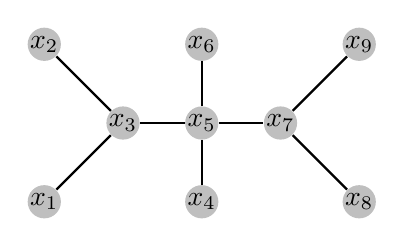
\begin{tikzpicture}[scale=1]
    % Draw a 7,11 network
    % First we draw the vertices
    \foreach \pos/\name in {{(1,1)/x_1}, {(1,3)/x_2}, {(2,2)/x_3}, {(3,1)/x_4}, {(3,2)/x_5}, {(3,3)/x_6}, {(4,2)/x_7}, {(5,1)/x_8}, {(5,3)/x_9}}
        \node[vertex] (\name) at \pos {$\name$};
    
    
    % Connect vertices with edges 
    \foreach \source/ \dest in {x_1/x_3, x_2/x_3,x_3/x_5,x_4/x_5, x_6/x_5, x_5/x_7, x_7/x_8, x_7/x_9}
        \path[edge] (\source) -- (\dest) ;
        
\end{tikzpicture}

\end{center}



\begin{center}
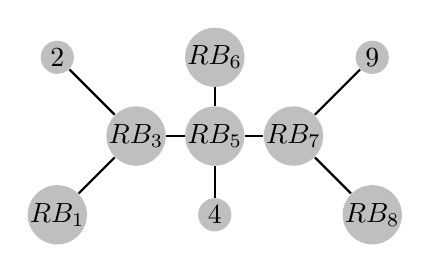
\begin{tikzpicture}[scale=1]
    % Draw a 7,11 network
    % First we draw the vertices
    \foreach \pos/\name in {{(1,1)/RB_1}, {(1,3)/2}, {(2,2)/RB_3}, {(3,1)/4}, {(3,2)/RB_5}, {(3,3)/RB_6}, {(4,2)/RB_7}, {(5,1)/RB_8}, {(5,3)/9}}
        \node[vertex] (\name) at \pos {$\name$};
    
    
    % Connect vertices with edges 
    \foreach \source/ \dest in {RB_1/RB_3, 2/RB_3,RB_3/RB_5,4/RB_5, RB_6/RB_5, RB_5/RB_7, RB_7/RB_8, RB_7/9}
        \path[edge] (\source) -- (\dest) ;
        
\end{tikzpicture}
\end{center}

Assume $X_{I^0_3}>X_{I^0_5}$ and $X_{I^0_7}>X_{I^0_5}$. Since that, Rebel 5 will get the information from Rebel 3,7 before he reports $I^0_5$. Since that, Rebel 5 has a profitable deviation by just reporting $\bar{I}^0_5=x_3\times x_5\times x_7<I^0_5$ to let Rebel 3, 7 think he is still in the path and to let the coordination to \textbf{revolt} be succeeded. Rebel 6 can detect such deviation since $\bar{I}^0_5$ did not include Rebel 6's own index $x_6$. However, if Rebel 6 form the off-path belief as Equation ~\ref{eq_grim_trigger}, he will then play \textbf{stay} forever although the coordination has been succeeded.

\end{example}

Due to the pay-off function is not strictly increasing with the number of \textbf{revolts}, some Rebels will be excluded from coordination with this grim-trigger-like strategies. As Example ~\ref{ex_deviation} shows, some strategies other than $I^t$ have to be considered as the strategies in the equilibrium path to avoid the situation where some Rebels are out of an existing coordination. The introducing of message $\langle 1 \rangle$ gives more equilibrium paths when grim trigger is adopted. 

\subsubsection{Sketch of the proof for Theorem ~\ref{thm_main_result}}

In the previous subsections, I have listed the belief updating in the proposed equilibrium path in Table ~\ref{Table_blf_up_reporting}, Table~\ref{Table_blf_up_cdt11}, and Table~\ref{Table_blf_up_cdt12}. Lemma ~\ref{lemma_in_the_path} show that such equilibrium path is APEX.
\begin{lemma}\label{lemma_in_the_path}
If the state has strong connectedness, then for all $n$-person repeated $k$-Threshold game with parameter $1\leq k\leq n$ played in any FFCCU network without cycles, there is an equilibrium path that is APEX.
\end{lemma}
\begin{proof}
The proof is in the Appendix.
\end{proof}


For the histories outside of equilibrium path, those histories could be detectable or undetectable. The proof for Theorem ~\ref{thm_main_result} is as follows. First, I use off-path belief to prevent players from making detectable deviations, such as deviations from playing the specified forms of sequences listed in Table ~\ref{Table_msg_reporting} and ~\ref{Table_msg_coordination}. Then I argue that any undetectable deviation made by a Rebel before he knows the relevant information, $\#[Rebels](\theta)\geq k$ or $\#[Rebels](\theta)< k$, will create noises in his own learning process to reduce his own expected continuation pay-off.  To see why a player's undetectable deviation will create noises to impede his own learning process before he knows the relevant information, we may consider the case in which a Rebel wants to mimic pivotal plays' behaviors by sending $\langle 1 \rangle$. According to Table ~\ref{Table_blf_up_cdt11} and Table ~\ref{Table_blf_up_cdt12}, his neighbors' continuation playing after observing $\langle 1 \rangle$ is to play \textbf{stay} forever or to play \textbf{revolt} forever. Since all his neighbors will repeat the same action afterward, he cannot get more information to learn about $\theta$. When $\delta$ is high enough, because he can learn the relevant information (by Lemma ~\ref{lemma_learn}) if he stays in the path, he can get better continuation payoff by staying in the path. This is because, by doing so, his payoff achieves the maximum static payoff as 1 when $\#[Rebels](\theta)\geq k$ as well as achieves the maximum static payoff as 0 when $\#[Rebels](\theta)< k$. Claim ~\ref{claim_can_not_pretend_almost_success} shows this argument.

\subsection{Discussion}
\label{sec:varies}


\subsubsection{Variation: Pay-off as signals}
The assumption on the observability of pay-off can be relaxed without change the result in Theorem ~\ref{thm_main_result}. One may consider a situation such that the static pay-off depends not only on joint efforts but also depends on other random effects, says the weather.\footnote{e.g.,\citep{SHADMEHR2011}}. Specifically, consider there is a public signal $y\in \{y_1,y_2\}$ generated by Rebels' actions. Let Rebel $i$'s pay-off function be $u_{Rebel}(a_{Rebel_i},y)$, and let $u_{Rebel}(\textbf{stay},y_1)=u_{Rebel}(\textbf{stay},y_2)=u_0$. The distribution of $y_1$ and $y_2$ is 
\begin{eqnarray*}
p_{1s} &=& \mathrm {Pr}(y=y_1|\#\textbf{revolt}\geq k) \\
p_{1f} &=& \mathrm {Pr}(y=y_1|\#\textbf{revolt}< k) \\
p_{2s} &=& \mathrm {Pr}(y=y_2|\#\textbf{revolt}\geq k) \\
p_{2f} &=& \mathrm {Pr}(y=y_2|\#\textbf{revolt}< k) 
\end{eqnarray*}
with
\begin{equation}
p_{1s}u_{Rebel}(\textbf{revolt}, y_1)+p_{2s}u_{Rebel}(\textbf{revolt}, y_2)>u_0>p_{1f}u_{Rebel}(\textbf{revolt}, y_1)+p_{2f}u_{Rebel}(\textbf{revolt}, y_2) \label{eqn_network_6}
\end{equation}
and
\begin{equation}
1>p_{1s}>0,1>p_{2s}>0,p_{1f}=1-p_{1s},p_{2f}=1-p_{2s} \label{eqn_network_7}
\end{equation}

Equation~\ref{eqn_network_6} is a generalization for the previous setting. Equation~\ref{eqn_network_7} is a full support assumption on signal $y$. 

We can construct exactly the same equilibrium strategies by ignoring the noisy signal $y$ when Equation~\ref{eqn_network_7} holds. By directly checking the equilibrium path constructed in previous sections (see also Table ~\ref{Table_msg_reporting} and ~\ref{Table_msg_coordination}), \textit{at most one} Rebel playing \textbf{revolt} in a period before some Rebels play $\langle 1 \rangle$, and thus the signal $y$ is not relevant before some Rebels play $\langle 1 \rangle$. Moreover, playing $\langle 1 \rangle$ comes from a Rebel's observation in reporting period where Rebels' strategies are independent from $y$, and thus playing $\langle 1 \rangle$ is independent from $y$. We then just check if a Rebel want to deviate to play $\langle 1 \rangle$ to get additional information coming from $y$. According to equilibrium strategies in the path, however, playing $\langle 1 \rangle$ will incur either coordination to \textbf{stay} or coordination to \textbf{revolt} after current block as Table ~\ref{Table_blf_up_cdt11} and Table ~\ref{Table_blf_up_cdt12} shows. Since signal $y$ is noisy, and since Rebels' actions will repeat, he can not learn the relevant information. As the same argument in Claim ~\ref{claim_can_not_pretend_almost_success}, he is better off by staying in the equilibrium path.

If Equation~\ref{eqn_network_7} does not hold, says $p_{1s}=p_{2f}=1$, then the signal $y$ is not noisy, and therefore the equilibrium constructed in the previous section is no longer an equilibrium. However, another APEX equilibrium can be constructed by letting all Rebels play \textbf{revolt} in the first period, and then keep playing \textbf{revolt} or \textbf{stay} contingent on the signals $y=y_1$ or $y=y_2$ when $\delta$ is sufficiently high.

\subsubsection{Variation: Rebels with different levels of efforts}

Consider a model in which players have different levels of efforts to contribute to a collective action. Let the set of states of nature be $\hat{\Theta}=\Theta \times \Xi$, where $\Xi=\{1,2,...,k\}^n$. Let $\hat{\theta}=(\theta,e)$, where $\theta\in \Theta$ and $e\in \Xi$. $\hat{\theta}$ is interpreted as a state of nature in which a player $i$ could be either a Rebel or Inert with $e_i$ efforts, where $e_i\in \{1,2,...,k\}$. When a Rebel $i$ plays \textbf{revolt}, he contributes $e_i$ efforts to a collective action, while the success of such collective action requires $k$ amount of efforts. If the collective action succeed, such Rebel $i$ will get $b_i>0$ as his reward. The pay-off structure is modified as the following.
\begin{enumerate}
\item $u_{Rebel_i}(a_{Rebel_i},a_{-\theta_i})=b_i$ if $a_{Rebel_i}=\textbf{revolt}$ and $\sum_{j:a_{\theta_j}=\textbf{revolt}}e_j\geq k$
\item $u_{Rebel_i}(a_{Rebel_i},a_{-\theta_i})=-e_i$ if $a_{Rebel_i}=\textbf{revolt}$ and $\sum_{j:a_{\theta_j}=\textbf{revolt}}e_j< k$
\item $u_{Rebel_i}(a_{Rebel_i},a_{-\theta_i})=0$ if $a_{Rebel_i}=\textbf{stay}$
\item $u_{Inert_i}(a_{Inert_i},a_{-\theta_i})=1$ if $a_{Inert_i}=\textbf{stay}$
\end{enumerate}

After the nature chooses a $\hat{\theta}$, players repeatedly play the above game in a network $G$. To see that the equilibrium constructed in previous section is still an equilibrium, transform the network and the state $(G,\hat{\theta})$ to $(G^{'},\hat{\theta}^{'})$ such that, in $(G^{'},\hat{\theta}^{'})$, there are $e_i$ different players attached to a single player $i$ for each $i\in N$, and all the players are with levels of efforts as 1. What matters here is that the states of nature are finite and discrete, and therefore we can use prime indexing to construct the equilibrium as previous section shows.


\subsubsection{Variation: networks with cycles}

The prime indexing can deal with a potential free problem when networks have cycles, although we may need to redefine the information hierarchy in order to redefine which Rebels are forced to report their private information. Consider the following Example ~\ref{ex_no_free_rider_cycle}.

\begin{example}
\label{ex_no_free_rider_cycle}
Let $k=6$. Rebel 3 and Rebel 4 have the same information $I^1_3=I^1_4$. Since reporting is costly, if there is no punishment, Rebel 3 (or Rebel 4) may shirk and deviate from truthfully reporting if Rebel 4 (or Rebel 3) can reports truthfully. However, this kind of deviation can be detected by Rebel 5 (or Rebel 2) since $I^1_3$ should be equal to $I^1_4$. 

\begin{center}
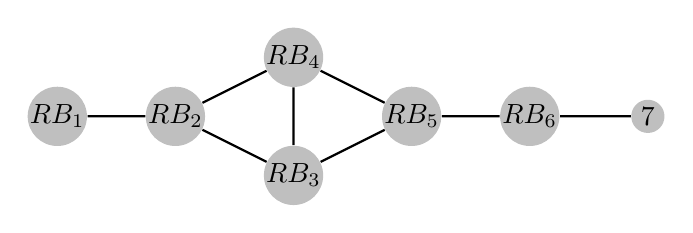
\begin{tikzpicture}[scale=1.5]
    % Draw a 7,11 network
    % First we draw the vertices
    \foreach \pos/\name in {{(1,2)/RB_1}, {(2,2)/RB_2}, {(3,1.5)/RB_3}, {(3,2.5)/RB_4}, {(4,2)/RB_5}, {(5,2)/RB_6}, {(6,2)/7}}
        \node[vertex] (\name) at \pos {$\name$};
    
    
    % Connect vertices with edges 
    \foreach \source/ \dest in {RB_1/RB_2, RB_2/RB_3,RB_2/RB_4,RB_3/RB_5, RB_4/RB_5, RB_5/RB_6, 7/RB_6, RB_4/RB_3}
        \path[edge] (\source) -- (\dest) ;
        
\end{tikzpicture}
\end{center}

\end{example}

Indeed, this monitoring technique will be less invalid if the network is not commonly known. In this example, if Rebels has asymmetric information about network structure, says Rebel 5 (or Rebel 2,3) does not certain about if there is a link between Rebel 4 and Rebel 2, then Rebel 4 can just pretend that he doesn't know Rebel 2\footnote{However, if there is asymmetric information about network structure, then Example ~\ref{ex_no_free_rider_cycle} is not exactly a free rider problem. Dependent on what asymmetric information is given, Rebel 3 and Rebel 4 then have different incentives in untruthful reporting. Untruthful reporting could be a dominant strategy for Rebel 4 but not necessary be a dominant strategy for Rebel 3.}. The analysis in incomplete information about network structure is beyond the scope of this paper. Recent paper such as \citep{Galeotti2010} deal with the issues when network is not commonly known.

There is another free rider problem which is harder to deal with. Remind that the implicit technique in my equilibrium construction is that the pivotal Rebels can be identified before the game enter into each reporting period in each block. When the networks has cycles, the selection of pivotal Rebels needs more elaboration. Consider Example ~\ref{ex_free_rider_cycle}.
\begin{example}\label{ex_free_rider_cycle}
Let $k=6$. Suppose the network and $\theta$ is as the following. 

\begin{center}
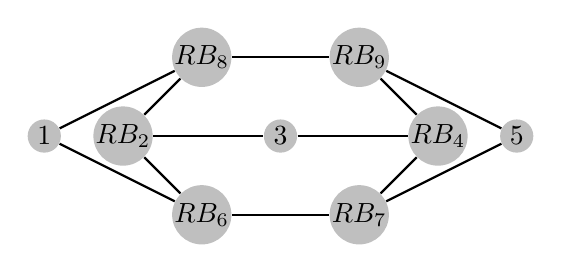
\begin{tikzpicture}[scale=1]
    % Draw a 7,11 network
    % First we draw the vertices
    \foreach \pos/\name in {{(1,3)/1}, {(2,3)/RB_2}, {(4,3)/3}, {(6,3)/RB_4}, {(7,3)/5}, {(3,2)/RB_6}, {(5,2)/RB_7}, {(3,4)/RB_8}, {(5,4)/RB_9}}
        \node[vertex] (\name) at \pos {$\name$};
    
    
    % Connect vertices with edges 
    \foreach \source/ \dest in { 1/RB_6, 1/RB_8, RB_2/3, RB_2/RB_8, 3/RB_4, RB_2/RB_6, RB_6/RB_7, RB_8/RB_9, RB_9/RB_4, RB_7/RB_4, RB_9/5, RB_7/5}
        \path[edge] (\source) -- (\dest) ;
        
\end{tikzpicture}
\end{center}

Assume that one round of reporting is done. Rebel 2 has known $\{RB_2,RB_6,RB_8,RB_9,RB_7\}$, Rebel 4 has known $\{RB_4,RB_7,RB_9,RB_8,RB_6\}$, and so on. One more round of reporting will let Rebels 3,6,7,4,9,8 know the true state $\theta$, and therefore Rebels 3,6,7,4,9,8 are all pivotal players. We may have a rule as Example ~\ref{ex_free_rider_tree} to pick up a pivotal Rebel, say we pick Rebel 4 before entering the next reporting period. However, this pivotal player selection is ex-post. The true state $\theta^{'}$ could be as the following.

\begin{center}
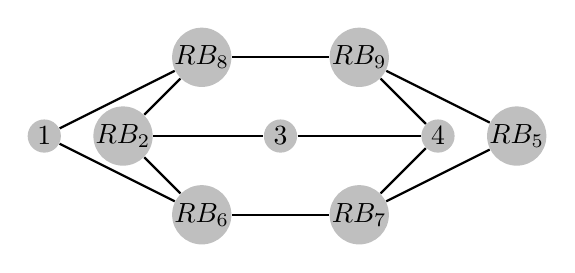
\begin{tikzpicture}[scale=1]
    % Draw a 7,11 network
    % First we draw the vertices
    \foreach \pos/\name in {{(1,3)/1}, {(2,3)/RB_2}, {(4,3)/3}, {(6,3)/4}, {(7,3)/RB_5}, {(3,2)/RB_6}, {(5,2)/RB_7}, {(3,4)/RB_8}, {(5,4)/RB_9}}
        \node[vertex] (\name) at \pos {$\name$};
    
    
    % Connect vertices with edges 
    \foreach \source/ \dest in { 1/RB_6, 1/RB_8, RB_2/3, RB_2/RB_8, 3/4, RB_2/RB_6, RB_6/RB_7, RB_8/RB_9, RB_9/4, RB_7/4, RB_9/RB_5, RB_7/RB_5}
        \path[edge] (\source) -- (\dest) ;
        
\end{tikzpicture}
\end{center}

Now node 4 is an Inert and so that he is not a pivotal Rebel. Some other rules are needed to be applied to select a pivotal Rebel (say, Rebel 5 in this case) during the game is played. 

\end{example}

As Example ~\ref{ex_free_rider_tree} or ~\ref{ex_free_rider_cycle} show, a free rider problem may occur if the selection of pivotal Rebels is not done before the game is played. When the networks has cycles, this problem seems more harsh and the selection rule may not be done before the game is played. Though it is possible to construct a selection rule, this rule is still infeasible in this paper. 

I leave a conjecture here and end this section.

\begin{conjecture}
For $n$-person repeated $k$-Threshold game with parameter $1\leq k < n$ played in any FFCCU network,
if the state $\theta$ has strong connectedness and $\pi(\{\theta: \theta\text{ has strong connectedness}\})=1$ with full support, then there is a $\delta$ such that there is a (weak) sequential equilibrium which is APEX.
\end{conjecture}



\section{Conclusion}
\label{sec:con}

I model a coordination game and illustrate the learning processes generated by strategies in a sequential equilibrium and answer the question proposed in the beginning: what kind of networks can conduct coordination in a collective action game with information barrier. In the equilibrium, players transmit the relevant information by encoding such information by their actions in the time horizontal line. Since there is an expected cost in coding information, potential free rider problems may occur to impede the learning process. When the networks are FFCCU without cycle, players can always learn the underlying relevant information and conduct the coordination only by their actions. However, what kinds of equilibrium strategies can constitute a learning process to learn the relevant information in cyclic networks still remains to be answered.


The construction of communication protocol exploits the assumption of finite type space and the finite threshold. Since the relevant information has been parameterized as a threshold, players can acquire this information by jointly incrementally reporting their own private information. The major punishment to keep players staying in the equilibrium path is then the joint shifting to play same actions as the stopping to update their information. The threshold model seems a general model in proofing that a communication protocol not only leads a learning process but also constitutes an equilibrium to reveal the relevant information in finite time.

Existing literatures in political science and sociology have recognized the importance of social network in influencing individual's behavior in participating social movements, e.g., \citep{Passy2003}\citep{McAdam2003}\citep{Siegel2009}. This paper views networks as routes for communication where rational individuals initially have local information, and they can influence nearby individuals by taking actions. Such influence may take long time to travel across individuals, and the whole process incurs inefficient outcomes in many periods. A characterization in the speed of information transmission across a network is not answered here, although it is an important topic in order to give more attentions in investigating the most efficient way to let the information be spread . This question would remain for the future research.



\bibliographystyle{abbrvnat}	% (uses file "plain.bst")
\bibliography{jmp_ref}		% expects file "myrefs.bib"


\appendix
\section{Appendix}

\noindent\textbf{proof for Lemma ~\ref{lemma_learn}}

\begin{proof}
The proof is done by contradiction. Suppose Rebels' strategies constitute an APEX. By definition of APEX, there is a time $T^{\theta}$ when actions start to repeat at state $\theta$. Let $T=\max_{\theta\in \Theta}{T^{\theta}}$. Pick that time $T_i=T+1$ and suppose the consequence did not not holds so that $0<\sum_{\theta:\#[Rebels](\theta)\geq k}\beta^{\pi,\tau^*}_{G_i}(\theta|h^{s}_{G_i})<1$ for some $s\geq T_i$. Then this Rebel puts some positive weights on some $\theta\in \{\theta:\#[Rebels](\theta)< k\}$ and puts some positive weights on $\theta\in \{\theta:\#[Rebels](\theta)\geq k\}$ at that time $s$. Note this Rebel $i$ has already known $\theta_j$ if $j\in G_i$, and therefore Rebel $i$ put some positive weights on $\theta\in \{\theta:\#[Rebels](\theta)< k, \theta_l=Rebel, l\notin G_i\}$ and $\theta\in \{\theta:\#[Rebels](\theta)< k, \theta_l=Inert, l\notin G_i\}$. Since actions start to repeat at $T$, all $i$'s neighbors will play the same actions as the actions at time $T$, but then Rebel $i$ can not update information from his neighborhood by Bayesian rule. Suppose $i$'s continuation strategy is to play \textbf{revolt} repeatedly, then this is not ex-post efficient if $\#[Rebels](\theta)< k$. Suppose $i$'s continuation strategy is to play \textbf{stay} repeatedly, then this is not ex-post efficient if $\#[Rebels](\theta)\geq k$
\end{proof}

\bigskip
\noindent\textbf{proof for Theorem ~\ref{lemma_empty}}

This proof follows three useful claims, Claim ~\ref{lemma_I_subset_N}, Claim ~\ref{lemma1} and Claim ~\ref{lemma_connected}. First note that $I^t_i$ and $N^t_i$, $t\geq 1$ can be expressed as 
\begin{equation}
\label{eq_info_nb}
I^{t}_i = \bigcup_{k_0\in G_i\cap R^{t}}\bigcup_{k_1\in G_{k_0}\cap R^{t-1}}...\bigcup_{k_{t-1}\in G_{k_{t-2}}\cap R^{1}}G_{k_{t-1}}\cap R^0
\end{equation}
, while $H^t_i$ can be expressed as
\begin{equation}
\label{eq_nb}
N^t_i = \bigcup_{k_0\in G_i\cap R^{t-1}}\bigcup_{k_1\in G_{k_0}\cap R^{t-2}}...\bigcup_{k_{t-2}\in G_{k_{t-3}}\cap R^{0}}G_{k_{t-2}}
\end{equation}

\begin{claim}
\label{lemma_I_subset_N}
$I^t_i\subset N^t_i$ for $t\geq 1$
\end{claim}
\begin{proof}
$I^t_0\subset N^t_0$ by definition. Since $R^t\subset R^{t-1}$ for $t\geq 1$, $I^t_i\subset N^t_i$ for $t\geq 1$ by comparing Equation ~\ref{eq_info_nb} and Equation ~\ref{eq_nb}.
\end{proof}

\begin{claim}
\label{lemma1}
If the network is FFCCU without cycle, then for each $t\geq 1$ block, we have $i\in R^t\Leftrightarrow i\in R^{t-1} \text{ and } \exists k_1,k_2\in R^{t-1}\cap \bar{G}_i$, where $k_1\neq k_2$.
\end{claim}
\begin{proof}
The proof is by induction. We first show that the statement is true for $t=1$. 

\textbf{Base}: $i\in R^1\Leftrightarrow [i\in R^0] \wedge [\exists k_1,k_2\in (R^0\cap \bar{G}_i)]$. 

$\Rightarrow$: Since $i\in R^1$, then $i\in R^0$ and then $I^0_i\nsubseteq N^0_j$ for all $j\in \bar{G}_i$ by definition. Since $I^0_i=R^0\cap G_i$, then $\forall j\in \bar{G}_i [\exists k\in (R^0\cap \bar{G}_i) [k\notin N^0_j]]$. Since the $j\in \bar{G}_i$ is arbitrary,  we then have a pair of $k_1, k_2 \in (R^0\cap \bar{G}_i)$ such that $k_1\notin N^0_{k_2}$ and $k_2\notin N^0_{k_1}$.

$\Leftarrow$: Pick $k\in \{k_1,k_2\}\subseteq (R^0\cap \bar{G}_i)$, and pick an arbitrary $j\in \bar{G}_i\backslash \{k\}$. Note that $k\notin N^0_j$, otherwise there is a cycle from $i$ to $i$. Hence $[k\in (R^0\cap \bar{G}_i)] \wedge [k\notin N^0_j]$ and therefore $[k\in I^0_i] \wedge [k\notin N^0_j]$. Then we have $I^0_i\nsubseteq N^0_j$ for arbitrary $j\in \bar{G}_i$, and thus $i\in R^1$.

\textbf{Induction hypothesis}: the statement is true for $\{1,2,..,t\}$ where $t\geq 1$. 


If the hypothesis is true, then $i\in R^{t+1}\Leftrightarrow [i\in R^{t}] \wedge [\exists k_1,k_2\in (R^{t}\cap \bar{G}_i)]$


$\Rightarrow$: since $i\in R^{t+1}$, then $i\in R^t$ and $I^t_i\nsubseteq N^t_j$ for all $j\in \bar{G}_i$ by definition. Recall that $I^t_i$ can be expressed as Equation ~\ref{eq_info_nb} and $H^t_i$ can be expressed as Equation ~\ref{eq_nb}, then for every $l\in I^{t-1}_i$, we can find a path connecting $i$ to $l$ by the induction hypothesis. If $j\in \bar{G}_i$, then we can find a path connecting $j$ to $l$ by connecting $j$ to $i$, and then connecting $i$ to $l$. Thus, if $l\in I^{t-1}_i$ then $l\in N^t_J$, and hence $I^{t-1}_i\subseteq N^t_{j}$ for all $j\in \bar{G}_i$. Recall that $I^t_i = \bigcup_{k\in N_i\cap R^t}I^{t-1}_k$ and $i\in R^{t+1}$, then we must have $\forall j\in \bar{G}_i [\exists k\in (R^t\cap \bar{G}_i)[ I^{t-1}_k\nsubseteq N^t_j]]$, since $I^{t-1}_i\subseteq N^t_{j}$. Note that such $j\in \bar{G}_i$ is arbitrary,  we then have a pair of $k_1, k_2 \in (R^{t}\cap \bar{G}_i)$ such that $k_1\notin N^t_{k_2}$ and $k_2\notin N^t_{k_1}$.
\bigskip

$\Leftarrow$:
By the induction hypothesis, we have a chain $k_{1_0},...,k_{1_t},i,k_{2_t},...,k_{2_0}$ with $k_{1_0}\in R^0$,..., $k_{1_t}\in R^t$, $i\in R^t$, $k_{2_t}\in R^t$,...,$k_{1_0}\in R^0$, where $k_{1_t},k_{2_t}\in (R^{t}\cap \bar{G}_i)$, $k_{1_0}\in I^{t-1}_{k_{1_t}}$ and $k_{2_0}\in I^{t-1}_{k_{2_t}}$. Note that $k_{1_0}\notin N^t_j$ whenever $j\in \bar{G}_i$, otherwise there is a cycle from $i$ to $i$ since $\{i,k_{2_t},...,k_{2_0}\}\in N^t_j$, and hence $[k_{1_0}\in I^{t-1}_{k_{1_t}}] \wedge [k_{1_0}\notin N^t_j]$ for all $j\in \bar{G}_i$. Therefore we have $[I^{t-1}_{k_{1_t}}\in I^t_i] \wedge [I^{t-1}_{k_{1_t}}\notin N^t_j]$ for all $j\in \bar{G}_i$ since $k_{1_t},k_{2_t}\in (R^{t}\cap \bar{G}_i)$ and $[k_{1_0}\in I^{t-1}_{k_{1_t}}] \wedge [k_{1_0}\notin N^t_j]$ for all $j\in \bar{G}_i$. Then we have $I^t_i=\bigcup_{k\in N_i\cap R^{t}}I^{t-1}_k\nsubseteq N^t_j$ for arbitrary $j\in \bar{G}_i$, and thus $i\in R^{t+1}$.



We can then conclude that the statement is true by induction.




\end{proof}



\begin{claim}
\label{lemma_connected}
If the network FFCCU without cycle and if the state has strong connectedness, then if there is a pair of $R^{t}$ nodes then there exists a $R^{t}$-path connecting them.
\end{claim}
\begin{proof}
The proof is by induction and by Claim ~\ref{lemma1}. Since the state has strong connectedness, we have a $R^0$-path connecting each pair of $R^0$ nodes. Since all pairs of $R^0$ nodes are connected by a $R^0$-path, then for all pairs of $R^1$ nodes must be in some of such paths by Claim ~\ref{lemma1}, and then connected by a $R^0$-path. But then all the $R^0$-nodes in such path are all $R^1$ nodes by Claim ~\ref{lemma1} again and by $R^t\subseteq R^{t-1}$ for $t\geq 1$ by definition. Thus, for all pairs of $R^1$ nodes has a $R^1$-path connecting them. The similar argument holds for $t> 1$, we then get the result.

\end{proof}
I begin to prove this Theorem ~\ref{lemma_empty}. I first claim that if $R^t\neq \emptyset$ and if $R^{t+1}= \emptyset$, then $R^0\subset I^t_i$ whenever $i\in R^t$. Then I claim that if $R^t\neq \emptyset$ then $\# R^{t+1}<\# R^t$. Finally, I iterate $R^t$ with $t\geq 0$ to get the conclusion.

If $R^t\neq \emptyset$ but $R^{t+1}= \emptyset$, I claim that $R^0\subset I^{t}_i$ for all $i\in R^t$. The proof is by contradiction. If $R^0\not\subset I^{t}_i$, there is a $j\in R^0$ but $j\notin I^t_i$. Since $I^t_i$ can be expressed as Equation ~\ref{eq_info_nb}, there is no such a path $\{i,k_0,k_1,...,k_{t-1},j\}$, where $k_0\in G_i\cap R^{t},k_1\in G_{k_0}\cap R^{t-1},...,k_{t-1}\in N_{k_{t-2}}\cap R^{1}$. Since $R^{t+1}=\emptyset$ and therefore $R^{t^{'}}=\emptyset$ if $t^{'}\geq t+1$, and hence there is no such a path containing a node in $R^{t^{'}}=\emptyset$, where $t^{'}\geq t+1$ connecting $i$ to $j$. But $i\in R^t$ and $i,j\in R^0$, if there is no such a path, then it violate either Claim ~\ref{lemma_connected} or Claim ~\ref{lemma1}. Contradiction.

Next I claim that if $R^t\neq \emptyset$ then $\# R^{t+1}<\# R^t$. The proof is the followings. Given a node $i$ in $R^t$, let $j\in R^t$ (could be $i$ itself) be the node connected with $i$ with the maximum shortest $R^t$ path. This $j$ can be found since $R^t\neq \emptyset$ and the network is finite. Then there is no $R^t$ node in $j$'s neighborhood other than the nodes in this path. Since the network is without cycle, there is at most one $R^t$ node in $j$'s neighborhood. But then $j\notin R^{t+1}$ since it violate Claim ~\ref{lemma1}.

Starting from $R^0\neq \emptyset$ and iterating $R^t$ with $t\geq 0$, if $R^t\neq \emptyset$ but $R^{t+1}= \emptyset$, then there is some $i$ with $R^0\subset I^t_i$ as the above paragraph shows; if $R^t\neq \emptyset$ and $R^{t+1}\neq \emptyset$, then we starting from $R^{t+1}$ and iterating $R^{t+1}$ with $t\geq t+1$. Since $\#R^{t+1}<\#R^t$ as the above paragraph shows, there is a time $t^{*}$ with $R^{t^{*}}=\emptyset$, then we get the conclusion.


\bigskip




\noindent\textbf{proof for Lemma ~\ref{lemma_at_most_two_nodes}}

\begin{proof}
Denote $(i,j)$-path as the set of paths from $i$ to $j$. The proof is by contradiction. Suppose there are three or more $R^t$-nodes in $C^t$, then pick any three nodes of them, and denote them as $i_1,i_2,i_3$. Let's say $i_2$ is in a $(i_1,i_3)$-path by strong connectedness, and therefore $i_2\in Tr_{i_1i_2}$ and $i_3\in Tr_{i_2i_3}$. First we show that $i_1\in G_{i_2}$ (or $i_3\in G_{i_2}$). Suppose $i_1\notin N_{i_2}$, since $i_1,i_2\in R^t$, then the $(i_1,i_2)$-path is a $R^t$-path by Claim ~\ref{lemma1}. Let this $(i_1i_2)$-path be $\{i_1,j_1,...,j_n,i_2\}$. Since $i_1,j_1,...,j_n,i_2\in R^t$, we then have $I^{t-1}_{i_1}\nsubseteq N^{t-1}_{j_1},...,I^{t-1}_{j_n}\nsubseteq N^{t-1}_{i_2}$ and $I^{t-1}_{j_1}\nsubseteq N^{t-1}_{i_1},...,I^{t-1}_{i_2}\nsubseteq N^{t-1}_{j_n}$. Since $I^{t-1}_{i_1}\subseteq N^{t-1}_{i_1},...,I^{t-1}_{i_2}\subseteq N^{t-1}_{i_2}$ by Claim ~\ref{lemma_I_subset_N}, we further have $\exists k_1\in R^0[k_1\in N^{t-1}_{j_1}\backslash I^{t-1}_{i_1}]$,...,$\exists k_n\in R^0[k_n\in N^{t-1}_{j_n}\backslash I^{t-1}_{i_2}]$. Since the state has strong connectedness, there is a $R^0$ path connecting $k_1,...,k_n$ by Claim ~\ref{lemma_connected}. But then we have already found $k_1,k_2$ such that $k_1\in N^{t-1}_{j_1}\backslash I^{t-1}_{i_1}$ and $k_2\in \bar{G}_{k_1}$. It is a contradiction that $i_1\in C$.

Now, $i_1,i_2,i_3$ will form a $R^t$-path as $\{i_1,i_2,i_3\}$. With the same argument as the above, we then have $\exists k_1\in R^0[k_1\in N^{t-1}_{i_2}\backslash I^{t-1}_{i_1}]$ and $\exists k_2\in R^0[k_2\in N^{t-1}_{i_3}\backslash I^{t-1}_{i_2}]$, and thus $i_1$ is not in $C$.
\end{proof}


\noindent\textbf{proof for Lemma ~\ref{lemma_no_node_outside}}
\begin{proof}
The proof is done by contradiction. Since $i\in R^t$, there is a $j\in (R^{t-1}\cap \bar{G}_i)$ by Lemma ~\ref{lemma1}. Note that $N^{t-1}_j\subseteq \bigcup_{k\in N^{t-1}_i}N_k$ since $N^{t-1}_j =\bigcup_{k\in I^{t-2}_j}N_k$, and $I^{t-2}_j\subseteq I^{t-1}_i\subseteq N^{t-1}_i$. If there is another node outside $\bigcup_{k\in N^{t-1}_i}N_k$ in $Tr_{ij}$, then there must be another node such that there is a path connected to some nodes in $N^{t-1}_j$ since the network is connected. It is a contradiction that $i\in C$.

\end{proof}

\subsection{Equilibrium}
\label{Apn_equilibrium}
\subsubsection{Out-off-path belief}

If Rebel $i$ detects a deviation at $m$ period, he form the belief as
\begin{equation}
\beta_{i}(\{\theta:\theta\in \times_{j\in G_i}\{\theta_j\}\times\{Inert\}^{n-\#G_i}\}|h^{m^{'}}_{G_i})=1 \text{ , } m^{'}\geq m
\end{equation}



\subsubsection{Equilibrium Path: Notations}


\begin{itemize}

\item $\langle \rangle_r$ be the set of finite sequences in which the action \textbf{r} occurs once and only once.
\item $PF(\langle \rangle,m)$ be the $m$-periods prefix of a finite sequence $\langle \rangle$.
\item $(i,j)$-path be the set of paths from $i$ to $j$.

\end{itemize}

\subsubsection{Equilibrium Path: reporting period}

\paragraph{reporting period: notations}
\begin{itemize}
\item $m$ be a period in reporting period in $t$ block.
\item $|\langle RP^t \rangle|$ be the total periods in reporting period in $t$-block
\item $O^{m,t}_i$ be the set of $i$'s neighbors $j$s who has played a sequence $M$ such that $M=PF(\langle I^{t-1}_j \rangle,m)$ and $M \in \langle \rangle_r$ at period $m$. 
\item $I^{m,t}_i\equiv (\bigcup_{k\in O^{m,t}_i} I^{t-1}_k)\cup I^{t-1}_i$ be the updated relevant information gathered by $i$ at period $m$. Note that $I^{0,t}_i=I^{t-1}_i$ and $I^{|\langle RP^t \rangle|,t }_i=I^{t}_i$.
\item $N^{m,t}_i\equiv (\bigcup_{k\in O^{m,t}_i} N^{t-1}_k)\cup N^{t-1}_i$
be the updated neighborhood which contains $I^{m,t}_i$

\item Let 
\[Ex_{I^{m,t}_i}\equiv \{l\notin N^{m,t}_i|\exists l^{'}\in I^{m,t}_i\text{ such that there exists a $(l,l^{'})$-path}\}\]
be all the possible Rebel nodes outside of $N^{m,t}_i$ given $I^{m,t}_i$
\item Let
\[Tr_{I^{m,t}_ij}\equiv Tr_{ij}\cap (Ex_{I^{m,t}_i}\cup I^{m,t}_i)\]
be all the possible Rebel nodes in the $Tr_{ij}$ given $I^{m,t}_i$. 
\end{itemize}
\paragraph{reporting period: automata}
\subparagraph{$i\notin R^{t}$}




\begin{itemize}
\item \textbf{WHILE LOOP}
\begin{itemize}
\item At $m\geq 0$, if $\#Ex_{I^{m,t}_i}\cup I^{m,t}_i< k$, report $\langle \textbf{stay} \rangle$ and then play \textbf{stay} forever.
\item Otherwise, \textbf{runs POST-CHECK }
\end{itemize}
\end{itemize}

\subparagraph{$i\in R^{t}$}

\begin{itemize}

\item \textbf{WHILE LOOP}
\begin{itemize}
\item At $m\geq 0$, if $\# Ex_{I^{m,t}_i}\cup I^{m,t}_i< k$, report $\langle \textbf{stay} \rangle$ and then play \textbf{stay} forever.
\item Otherwise, \textbf{runs MAIN }
\end{itemize}


\item \textbf{MAIN}

At $m\geq 0$, 

\begin{enumerate}
\item At $m=0$ and if $\# I^{t-1}_i=\# I^{0,t}_i= k-1$, then 
\textbf{runs POST-CHECK }


\item At $m=0$ and if $i\in R^t$ and
\[\nexists j\in R^{t-1}\cap\bar{G}_i \text{ such that }\exists l_1,l_2\in Tr_{ij}[[l_1\in N^{t-1}_j\backslash I^{t-1}_i] \wedge [l_2\in \bar{G}_{l_1}]]]\]
, then runs \textbf{CHECK.$0$}. Otherwise, recall \textbf{MAIN}
\item At $0\leq m \leq |RP^t|-|\langle I^{t-1}_i \rangle|$, play
\[\textbf{stay}\]
\item At $m = |RP^t|-|\langle I^{t-1}_i \rangle|+1$, then
\begin{enumerate}
\item if $O^{m,t}_i= \emptyset$ 
, then report
\[\langle I^{t-1}_i \rangle\]
\item if $O^{m,t}_i\neq \emptyset$, then \textbf{runs CHECK.k}

\end{enumerate}

\end{enumerate}





\item \textbf{CHECK.$0$}

At $m=0$, if $i\in C^t$, i.e. if $i\in R^t$ and
\[\nexists j\in R^{t-1}\cap \bar{G}_i \text{ such that }[\exists l_1,l_2\in Tr_{ij}[[l_1\in N^{t-1}_j\setminus I^{t-1}_i] \wedge [l_2\in \bar{G}_{l_1}]]]\]
, then
\begin{enumerate}
\item If $\#C^t=1$
, then 
\textbf{runs POST-CHECK }

\item If $\#C^t=2$, then denote $i_1,i_2\in C$ such that $I^{t-2}_{i_1}<I^{t-2}_{i_2}$, and then
\begin{itemize}
\item if $i=i_1$, then 
\textbf{runs POST-CHECK }
\item if $i=i_2$, then report
\[\langle I^{t-1}_i \rangle\]

\end{itemize}
\end{enumerate}




\item \textbf{CHECK.$m$}

 At $m>0$, if $O^{m,t}_i\neq \emptyset$, then there are two cases, 
\begin{enumerate}
\item Case 1: If $i\in R^t$ and 
\[\exists j\in  O^m_i \text{ such that }\exists l_1,l_2\in Tr_{I^{m,t}_ij}[[l_1\in I^{t-1}_j\backslash I^{t-1}_i] \wedge [l_2\in \bar{G}_{l_1}]]]\]
, then report 
\[\langle I^{t-1}_i \rangle\]
\item Case 2: If $i\in R^t$ and 
\[\not\exists j\in  O^m_i \text{ such that }\exists l_1,l_2\in Tr_{I^{m,t}_ij}[[l_1\in I^{t-1}_j\backslash I^{t-1}_i] \wedge [l_2\in \bar{G}_{l_1}]]]\]

\begin{enumerate}
\item Case 2.1: If $i\in R^t$ and 
\[\not\exists j\in R^{t-1}\cap (G_i\backslash  O^{m,t}_i) \text{ such that }[\exists l_1,l_2\in Tr_{I^{m,t}_ij}[[l_1\in N^{t-1}_j\backslash I^{t-1}_i] \wedge [l_2\in \bar{G}_{l_2}]]]\]
\[\textbf{Note: this case is the case when $i\in C$, thus recall Check.0}\]

\item Case 2.2: If $i\in R^t$ and 
\[\exists j\in R^{t-1}\cap (G_i\backslash  O^{m,t}_i) \text{ such that }[\exists l_1,l_2\in Tr_{I^{m,t}_ij}[[l_1\in N^{t-1}_j\backslash I^{t-1}_i] \wedge [l_2\in \bar{G}_{l_2}]]]\]

\begin{itemize}
\item if $\# I^{m,t}_i= k-1$
, then 
\textbf{runs POST-CHECK }

\item if $\# I^{m,t}_i< k-1$
, then report 
\[\langle I^{t-1}_i \rangle\]
\end{itemize}





\end{enumerate}

\end{enumerate}





\item \textbf{CHECK.k}

At $m\geq 1$, 
\begin{enumerate}


\item $O^{m,t}_i\neq \emptyset$, and
 \[\# I^{m,t}_i\geq k\]
, then 
\textbf{runs POST-CHECK }

\item $O^{m,t}_i\neq \emptyset$, and 
\[ \#I^{m,t}_i< k\]
, then \textbf{runs CHECK.$m$}
\end{enumerate}


\item \textbf{POST-CHECK}

\begin{enumerate}


\item At $m=|RP^t|$, then
\begin{enumerate}
\item If $i\in R^t$ and if $|I^{m,t}_i|\geq k-1$, then play
\textbf{revolt}

\item if $i\notin R^t$, then play
\textbf{stay}


\end{enumerate}
\end{enumerate}


\end{itemize}



\subsubsection{Equilibrium path: coordination period}
\paragraph{coordination period: notations}
\begin{itemize}
\item $m$ be a sub-block in coordination period.
\item Let 
\[Ex_{I^{t}_i}\equiv \{l\notin I^{t}_i|\exists l^{'}\in I^{t}_i\setminus I^{t-1}\text{ such that there exists a $(l,l^{'})$-path}\}\]
be all the possible Rebel nodes outside of $N^{t}_i$ given $I^{t}_i$.

\item Let
\[Tr_{I^{t}_ij}\equiv Tr_{ij}\cap (Ex_{I^{t}_i}\cup I^{t}_i)\]
be the set of possible Rebel nodes in the $Tr_{ij}$ given $I^{t}_i$. 

\end{itemize}




\paragraph{coordination period: automata}


\begin{itemize}





\item \textbf{1st Division} 

In 1st division, for $t=0$ block,

\begin{itemize}



\item If $\# Ex_{I^{t}_i}\cup I^{t}_i<k$, then play \textbf{stay} forever.

\item If $\# Ex_{I^{t}_i}\cup I^{t}_i \geq k$, and if $i\not\in R^1$, then play
\[\langle \textbf{stay} \rangle\]

\item If $\# Ex_{I^{t}_i}\cup I^{t}_i \geq k$, and if $i\in R^1$, then play
\[\langle x_i \rangle\]


\end{itemize}

In 1st division, for $t>0$ block and for $1\leq m \leq n$ sub-block,
\begin{itemize}

\item If $i$ has played $\langle 1 \rangle$, then play 
\[\langle x_i \rangle\]

\item If $\# Ex_{I^{t}_i}\cup I^{t}_i<k$, then play \textbf{stay} forever.

\item If $\# Ex_{I^{t}_i}\cup I^{t}_i\geq k$, and there are some $j\in \bar{G}_i$ have played $\langle \textbf{stay} \rangle $, then play
\textbf{stay} forever.
\item If $\# Ex_{I^{t}_i}\cup I^{t}_i \geq k$, and there is no $j\in \bar{G}_i$ has played $\langle \textbf{stay} \rangle $, then play
\[\langle x_i \rangle\]

\end{itemize}




\item \textbf{2nd Division} 

In $t=0$ block
\begin{itemize}
\item If $i\notin R^1$, play \[\langle \textbf{stay} \rangle \].
\item If $i\in R^1$, and if $\#I^0_i\geq k$, play \[\langle \textbf{stay} \rangle \].
\item If $i\in R^1$, if $\#I^0_i< k$, if $\# Ex_{I^{t}_i}\cup I^{t}_i\geq k$ and if some $j\in \bar{G}_i$ have played play $\mathbf{1}_j$ in the 1st division, then play \[\langle \textbf{stay} \rangle \].
\item If $i\in R^1$, if $\#I^0_i< k$, if $\# Ex_{I^{t}_i}\cup I^{t}_i\geq k$ and if no $j\in \bar{G}_i$ has played play $\mathbf{1}_j$ in the 1st division, then play \textbf{stay} forever.

\end{itemize}


In $t>0$ block, if there is no $j\in G_i$ such that $j$ has played $\langle \textbf{stay} \rangle$ in the \textbf{1st Division} , then run the following automata. Otherwise, play \textbf{stay} forever.

\begin{itemize}
\item $i\notin R^t $
\begin{itemize}
\item In the $1$-sub-block: play
\[\langle \textbf{stay} \rangle \]


\item In the $2\leq m\leq t+1$ sub-blocks: 

\begin{enumerate}

\item If $i\in R^{t^{'}}$ for some $t^{'}\geq 0$ and if there is a $j\in R^{t^{'}+1}\cap \bar{G}_i$ has played 
\begin{enumerate}
\item $\langle \textbf{stay} \rangle $ in $m=1$ sub-block
\item or $\langle \mathbf{1}_j \rangle$ in $m\geq 2$ sub-blocks
\end{enumerate}
, then play 
\[\langle x_i \rangle\] in $m+1$ sub-block.

\item Otherwise, play
\[\langle \textbf{stay} \rangle\] in current sub-block
\end{enumerate}

\end{itemize}

\item $i\in R^t$

\begin{itemize}
\item In the $1$-sub-block:
\begin{enumerate}
\item If $i$ has played $\langle 1 \rangle$, then play
\[\langle \textbf{stay} \rangle \]

\item If $i$ has not played $\langle 1 \rangle$ and if there is a $j\in \bar{G}_i$ has played $\langle 1 \rangle$, then play
\[\langle \textbf{stay} \rangle \]

\item If $i$ has not played $\langle 1 \rangle$ and if there is no $j\in \bar{G}_i$ has played $\langle 1 \rangle$, then
\begin{itemize}
\item If $\# I^{|RP^t|,t}_i\geq k$, then play
\[\langle \textbf{stay} \rangle \]
\item If $\# I^{|RP^t|,t}_i< k$, then play
\[\langle \mathbf{1}_i  \rangle \]
\end{itemize}

\end{enumerate}

\item In the $m\geq 2$-sub-block: 

\begin{enumerate}

\item If $i\in R^{t^{'}}$ for some $t^{'}\geq 0$ and if there is a $j\in R^{t^{'}}\cap \bar{G}_i$ has played 
\begin{enumerate}
\item $\langle \textbf{stay} \rangle$ in $m=1$ sub-block, or
\item $\langle \mathbf{1}_j \rangle$ in $m\geq 2$ sub-blocks
\end{enumerate}
, then play 
\[\langle x_i \rangle\] in $m+1$ sub-block.
\item Otherwise, play
\[\langle \textbf{stay} \rangle\] in current sub-block.
\end{enumerate}

\end{itemize}

\end{itemize}



\item \textbf{3rd Division} 

\begin{enumerate}
\item \textbf{INITIATING} 

If $i$ has observed $j\in \bar{G}_i$ has played
\begin{enumerate}
\item $\langle \textbf{stay} \rangle$ in $1$-sub-block in \textbf{2nd Division}  or
\item $\langle \mathbf{1}_j \rangle$ in $m\geq 2$ sub-blocks \textbf{2nd Division}  or
\item \textbf{s} in the \textbf{3rd Division} 
\end{enumerate}
, then play \textbf{revolt} forever

\item \textbf{NOT INITIATING} 

Otherwise, play 
\textbf{stay} 
in current period.
\end{enumerate}
\end{itemize}





\subsubsection{Proof for Theorem ~\ref{thm_main_result}}


The proof is organized as the following. In Claim ~\ref{claim_either_success_or_fail} and Lemma ~\ref{lemma_in_the_path}, we show that a Rebel will learn $\#[Rebels](\theta)\geq k$ or $\#[Rebels](\theta)< k$ in the equilibrium path. Lemma ~\ref{lemma_in_the_path} also show that the equilibrium path is ex-post efficient. Since that, there is a time $T$ such that a Rebel's static pay-off after $T$ is $1$ if $\#[Rebels](\theta)\geq k$ or $0$ if $\#[Rebels](\theta)\geq k$. Such pay-offs after time $T$ is the maximum static pay-off contingent on $\theta$. In Claim ~\ref{claim_detection_reporting_period}, I show that if a Rebel makes detectable deviation, then there is a positive probability event $E$ (by the full support assumption) contingent on this deviation such that his expected continuation static pay-off is strictly lower than that in equilibrium path after $T$. Finally, in Claim ~\ref{claim_deviation_higher_reporting}, Claim ~\ref{claim_can_not_pretend_almost_success}, Claim ~\ref{claim_must_report_1}, and Claim ~\ref{claim_report_with_no_message_coordination_period}, I show that if a Rebel makes undetectable deviation, then there is a positive event $E$ (by the full support assumption) contingent on this deviation such that his expected continuation static pay-off is also strictly lower than that in equilibrium path after $T$. Since the static pay-off after $T$ is maximum for all $\theta$ in equilibrium path, there is a $\delta$ such that a Rebel will not deviate. I then conclude this theorem.

To simplify the notations, if $P(\theta)$ is a property of $\theta$, then I abuse the notations by letting $\beta^{\pi,\tau^*}_{G_i}(P(\theta)|h^{m}_{G_i})\equiv \sum_{\theta:P(\theta)}\beta^{\pi,\tau^*}_{G_i}(\theta|h^{m}_{G_i})$. I also say ``$i$ knows $P(\theta)$'' to mean $\beta^{\pi,\tau^*}_{G_i}(P(\theta)|h^{m}_{G_i})=1$. 




\begin{claim}
\label{claim_either_success_or_fail}
In the equilibrium path and for $\#Ex_{I^{m,t}_i}\cup I^{m,t}_i\geq k$, where $m$ is a period in reporting period. If $i$ report $\langle 1 \rangle$, then either Rebels coordinate to \textbf{revolt} after $t$-block or $\# R^0<k$.
\end{claim}
\begin{proof}
By directly checking the equilibrium path, we have
\begin{enumerate}
\item if $\# I^{|RP^t|,t}_i\geq k$, then the coordination can be initiated by such $i$.
\item if $\# I^{|RP^t|,t}_i= k-1$, and if there is one more node who reported $\langle 1 \rangle$, then the coordination can be initiated by $i$.
\item if $\# I^{|RP^t|,t}_i= k-1$, and if there are no nodes who reported in current reporting period, then $\# I^{|RP^t|,t}_i=\# I^{t}_i= k-1$. We now check the conditions guiding $i$ to \textbf{POST-CHECK}.
\begin{itemize}
\item If $i$ is coming from the conditions in \textbf{MAIN}, it means that there are no further Rebels outside $I^{t-1}_i$, thus outside $\bigcup_{k\in I^{t-1}_i}G_k$.
\item If $i$ is coming from the conditions in \textbf{CHECK.0}, it means that there are no further Rebels outside $\bigcup_{k\in I^{t-1}_i}G_k\cap R^0$, and thus outside $\bigcup_{k\in I^{t-1}_i}G_k$. 
\item If $i$ is coming from the conditions in \textbf{CHECK.m}, it means that there are no further Rebels outside $\bigcup_{k\in I^{t-1}_i}G_k\cap R^0$, and thus outside $\bigcup_{k\in I^{t-1}_i}G_k$. 
\end{itemize}
Since $I^t_i=\bigcup_{k\in I^{t-1}_i}G_k\cap R^0 \subset \bigcup_{k\in I^{t-1}_i}G_k$ and $\#I^t_i<k$, and hence $\# R^0<k$.

\end{enumerate}


\end{proof}




\noindent \textbf{proof for Lemma ~\ref{lemma_in_the_path}}
\begin{proof}
We want to show that when $\theta$ satisfying $\#[Rebels](\theta)\geq k$, all the Rebels play \textbf{revolt} eventually; when $\theta$ satisfying $\#[Rebels](\theta)< k$, all the Rebels play \textbf{stay} eventually.
\begin{enumerate}
\item If all the Rebels only play $\langle I^{t-1} \rangle$ or $\langle \textbf{stay} \rangle$ in reporting period for all $t\geq 1$ block, then by the equilibrium path, those nodes played $\langle I^{t-1} \rangle$ are $R^t$-node, and those nodes played $\langle \textbf{stay} \rangle$ are non-$R^t$ nodes. 

If there are some Rebels play $\langle \textbf{stay} \rangle$ in $CD^t_{1,1}$, then all the Rebels play \textbf{stay} eventually; If $R^t$ Rebels play $\langle \textbf{stay} \rangle$ in $CD^t_{1,2}$, then all the Rebels will play \textbf{revolt} after third division in coordination period in this block. Otherwise, all the Rebels go to the next reporting period.

By Theorem ~\ref{lemma_empty}, there is a $t^{*}$ such that there is a $R^{t^{*}}$ node knows $\theta$, and therefore he knows if $\theta$ satisfying $\#[Rebels](\theta)\geq k$ or $\#[Rebels](\theta)< k$. In equilibrium path, such node play $\langle \textbf{stay} \rangle$ either in $CD^{t^{*}}_{1,1}$ or in $CD^{t^{*}}_{1,2}$. Thus the equilibrium path is APEX.

\item If there are some Rebels play $\langle 1 \rangle$ in reporting period for a $t\geq 1$ block, then by Claim ~\ref{claim_either_success_or_fail}, such nodes will knows if $\theta$ satisfying $\#[Rebels](\theta)\geq k$ or $\#[Rebels](\theta)< k$ after reporting period in this $t$-block. Then $\langle \textbf{stay} \rangle$ is either played in the first sub-block in first division or played in the first sub-block in second division in coordination period. Thus the equilibrium path is APEX.

 
\end{enumerate}

\end{proof}



Next, I prepare the claims to show that a Rebel will not deviate. I start with Claim ~\ref{claim_detection_reporting_period} in which the deviation is detectable.


\begin{claim} 
\label{claim_detection_reporting_period}
For $\#Ex_{I^{m,t}_i}\cup I^{m,t}_i\geq k$, where $m$ is a period. Denote $D$ be the set of Rebels who detect $i$'s deviation. If $\# I^{m,t}_i<k$ and if $D\neq \emptyset$, then there is a $\delta$ such that $i$ will not deviate.
\end{claim}
\begin{proof}

Denote $D$ be the set of neighbors who detect $i$'s deviation. Let the events be
\begin{eqnarray*}
E_1 	&= &\{\theta: \#[Rebels](\theta)< k\}\\
E_2 	&= &\{\theta: k\leq \#[Rebels](\theta)<k+\# D\}\\
E_3 	&= &\{\theta: \#[Rebels](\theta)\geq k+\# D\}
\end{eqnarray*}

In equilibrium path, there are periods $t^{s}$ ($t^{f}$) such that if $\theta$ satisfying $\#[\text{Rebels}](\theta)\geq k$ ( $\#[\text{Rebels}](\theta)< k$) then Rebels play \textbf{revolt} (\textbf{stay}) forever. If $i$ follows the equilibrium path, the expected static pay-off after $\max\{t^s,t^f\}$\footnote{There is $t^{s}$ or $t^{f}$ for each $\theta$. The maximum is among those possible $\theta$.} is
 \[\beta_{i}(E_2|h^{m}_{N_i})+\beta_{i}(E_3|h^{m}_{N_i})\]

If $i$ deviate, the expected static pay-off after $\max\{t^s,t^f\}$ is
 \[\beta_{i}(E_3|h^{m}_{N_i})\]
 
Therefore there is a loss in expected static pay-off of
\[\beta_{i}(E_2|h^{m}_{N_i})\]

Thus, there is a loss in expected continuation pay-off contingent on $E_2$ by
\[\delta^{\max\{t^s,t^f\}}\frac{\beta_{i}(E_2|h^{m}_{N_i})}{1-\delta}\]

Note that $\beta_{i}(E_2|h^{m}_{N_i})>0$, since $\#Ex_{I^{m,t}_i}\cup I^{m,t}_i\geq k$ and therefore $\beta_{i}(\#[Rebels](\theta)\geq k|h^{m}_{N_i})>0$ by full support assumption.
\end{proof}


Next, I prepare the claims to show that a Rebel will not deviate if such deviation is undetectable.

\begin{claim} 
\label{claim_deviation_higher_reporting}
In reporting period for $\# Ex_{I^{m,t}_i}\cup I^{m,t}_i \geq k$, if $\# I^{m,t}_i<k$, then there is a $\delta$ such that $i$ will not deviate by reporting $\bar{I}^{t-1}_i\neq I^{t-1}_i$ if such deviation is not detected by $i$'s neighbor.
\end{claim}

\begin{proof}
Assume $\bar{I}^{t-1}_i\neq I^{t-1}_i$. Since a detection of deviation has not occur, it must be the case that there is a non-empty set $F=\{j\in \bar{I}^{t-1}_i:\theta_j=Inerts\}$\footnote{Otherwise, there is a detection of deviation. Recall the definition in information hierarchy: $I^{-1}_i\subset I^{0}_i\subset...\subset I^{t-1}_i$ for all $i\in R^0$}. 


Let the set 
\[E_1=\{\bar{\theta}: \bar{\theta}_j=Rebel \text{ if } j\in F \text { and }\bar{\theta}_j=\theta_j \text{ if } j\notin F\}\]
be the set of pseudo events by changing $\theta_j$ where $j\in F$. And let
\[E_2=\{\theta: \theta_j=Inert \text{ if }j\in F \text { and }\bar{\theta}_j=\theta_j \text{ if } j\notin F\}\]
be the set of true event.

Then consider the event
\begin{eqnarray*}
E 	&= &\{\bar{\theta}\in E_1: \#[Rebels](\bar{\theta})\geq k\}\\
 	&= &\{\theta\in E_2: \#[Rebels](\theta)\geq k-\#F\}
\end{eqnarray*}

Partition $E$ as sub events
\begin{eqnarray*}
E_3 	&= &\{\theta\in E_2: \#[Rebels](\theta)\geq k\}\\
E_4 	&= &\{\theta\in E_2: k>\#[Rebels](\theta)\geq k-\#F\}
\end{eqnarray*}

By Lemma ~\ref{lemma_empty} and following the strategies in equilibrium path (since $i$ have not been detected), there is a block $\bar{t}^{s}$ with respect to $\bar{\theta}$ such that if $\bar{\theta}\in E$ then there some $R^{\bar{t}^s}$ Rebel $j$s, says $J$, will initiate the coordination, and then Rebels play \textbf{revolt} forever after $\bar{t}^s$-block. Note that such $j$ is with $\# {I}^{\bar{t}^{s}}_i \geq k$ by checking the equilibrium path.

We have several cases:
\begin{enumerate}
\item Case 1: If $i\in J$, his own initiation will only depends on $\# I^{\bar{t}^s}_i$ by Claim ~\ref{claim_can_not_pretend_almost_success} and Claim ~\ref{claim_must_report_1}, which is the same as he has reported $\langle {I}^{t-1}_i\rangle$. He is strictly better off by not deviating since playing $\langle\bar{I}^{t-1}_i\rangle$ is more costly than $\langle\bar{I}^{t-1}_i\rangle$ (since $X_{\bar{I}^{t-1}_i}>X_{I^{t-1}_i}$).

\item Case 2: If there is another $j$ such that $\bar{I}^{t-1}_i\not\subset I^{\bar{t}^{s}}_j$, then since such $j$'s initiation of coordination dependent on his own information $I^{\bar{t}^{s}}_j$ by Claim ~\ref{claim_can_not_pretend_almost_success} and Claim ~\ref{claim_must_report_1}, and $i$'s deviation did not change $j$'s information. It is strictly better by not deviating since playing $\langle\bar{I}^{t-1}_i\rangle$ is more costly than $\langle\bar{I}^{t-1}_i\rangle$ (since $X_{\bar{I}^{t-1}_i}>X_{I^{t-1}_i}$).

\item Case 3: Suppose there is another $j$ such that $\bar{I}^{t-1}_i\subset {I}^{\bar{t}^{s}}_j$ and $\# I^{\bar{t}^s}_i\geq k$, then such $j$ will initiate  the coordination to \textbf{revolt}. If $i$ did not follow $j$'s initiation of coordination, then there is a detection of deviation by checking the equilibrium path. $i$ will not deviate as Claim ~\ref{claim_detection_reporting_period} shows. If $i$ follows, and $\#I^{\bar{t}^s}_i\geq s$, we are in the Case 1. If $i$ follows, but $\#I^{\bar{t}^s}_i< s$, then $i$'s expected static pay-off after $\bar{t}^{s}$ is at most
\[
{\max\{\beta_{i}(E_3|h^{m}_{N_i})\times 1+\beta_{i}(E_4|h^{m}_{N_i})\times (-1), 0\}}
\]

However, if $i$ follow the equilibrium path, there is are $t^s$, $t^f$ such that the expected static pay-off after $\max\{t^s,t^f\}$ is
\[\max\{\beta_{i}(E_3|h^{m^{'}}_{N_i}),0\}\]

Thus, there is a loss in expected continuation pay-off contingent on $E$ by
\[\delta^{\max\{t^s,t^f\}}\frac{\min\{\beta_{i}(E_3|h^{m}_{G_i}),\beta_{i}(E_4|h^{m}_{G_i})\}}{1-\delta}\]
\end{enumerate}

Note that $\beta_{i}(E_3|h^{m}_{N_i})>0$ and $\beta_{i}(E_3|h^{m}_{N_i})>0$, since $\#Ex_{I^{m,t}_i}\cup I^{m,t}_i\geq k$ and $\# I^{m,t}_i<k$, and therefore $1>\beta_{i}(\#[Rebels](\theta)\geq k|h^{m}_{N_i})>0$ by full support assumption.
\end{proof}



\begin{claim} 
\label{claim_can_not_pretend_almost_success}
In reporting period for $\#Ex_{I^{m,t}_i}\cup I^{m,t}_i\geq k$, if $\#I^{m,t}_i\leq k-1$ and if $i\notin C^t$ or $i$ did not satisfy the condition to play $\langle 1 \rangle$ in equilibrium path, then $i$ will not play $\langle 1 \rangle$.
\end{claim}


\begin{proof}


Let
\[E^{'}=\{\theta:\#I^{RP^t,t}_i\leq k-1\}\]
. Note that such event is not empty by checking the timing where $i$ deviated:
\begin{enumerate}
\item If $i$ has a neighbor $j\in C^t$, then $j\not\in O^{RP^t,t}_i$, and therefore we can construct $E^{'}$ by assuming that all other neighbors (other than $i,j$ and other than $l\in O^{m,t}_i$) are non-$R^t$.
\item If \[\exists j\in R^{t-1}\cap \bar{G}_i \text{ such that } \exists k_1,k_2\in Tr_{ij}[[k_1\in N^{t-1}_j\backslash I^{t-1}_i] \wedge [k_2\in \bar{G}_{k_2}]]\], then just let $E^{'}=\{\theta: N^t_i\cap R^0\leq k-1\}=\{\theta: I^t_i\leq k-1\}$\footnote{note that $I^t_i$=$I^{RP^t,t}_i$}.
\end{enumerate}

Next, let 
\begin{eqnarray*}
E_1&=&\{\theta: \#[Reble](\theta)<k\}\cap E^{'}\\
E_2&=&\{\theta: \#[Reble](\theta)\geq k\}\cap E^{'}\\
\end{eqnarray*}

Note that $E_1$ and $E_2$ are not empty. According to equilibrium path, if $i$ did not follow the conditions to play $\langle 1 \rangle$, it must be the case that there are some nodes outside $I^t_i$ but there is a path consisting of Rebels to connect them. By strong connectedness, $E_1$ and $E_2$ are not empty.

Since $i$ deviate to play $\langle 1 \rangle$, his behavior after $CD^t_{1,1}$ will decide the following three cases:
\begin{enumerate}
\item If $i$ play $\langle \textbf{stay} \rangle$ in $CD^t_{1,1}$, then the coordination to \textbf{stay} starts after $CD^t_{1,1}$.
\item If $i$ play $\langle x_i \rangle$ in $CD^t_{1,1}$, then the coordination to \textbf{revolt} will be initiate after $CD^t_{1,2}$ if he mimic the behavior of a pivotal player (i.e., by mimicking those players who played $\langle 1 \rangle$ in equilibrium path).
\item If $i$ play $\langle x_i \rangle$ in $CD^t_{1,1}$, but he did not mimic the behavior of pivotal player, then such deviation will be detected.
\end{enumerate}

Thus, $i$'s expected static pay-off after the coordination period in this $t$-block is at most 
\[
{\max\{\beta_{i}(E_2|h^{m}_{N_i})\times 1+\beta_{i}(E_1|h^{m}_{N_i})\times (-1), 0\}}
\]

However, if he stay in the equilibrium, there is a $t^s$ ($t^f$) such that Rebels play \textbf{revolt} (\textbf{stay}) contingent on $E_2$ ($E_1$), and thus after $t^*=\max\{t^s,t^f\}$ he get the expected pay-off as
\[
{\max\{\beta_{i}(E_2|h^{m}_{N_i})\times 1, 0\}}
\]

After some calculation, after $t^*$, there is a loss of
\[\delta^{t^{*}}\frac{\min\{\beta_{i}(E_2|h^{m}_{G_i}),\beta_{i}(E_1|h^{m}_{G_i})\}}{1-\delta}\]
 



Note that $\beta_{i}(E_1|h^{m}_{N_i})>0$ and $\beta_{i}(E_2|h^{m}_{N_i})>0$, by $E_1$ and $E_2$ are not empty and by full support assumption.


\end{proof}







\begin{claim}
\label{claim_must_report_1}
In reporting period for $\beta_{i}(\#[Rebels](\theta)\geq k|h^{RP^t-1}_{G_i})>0$,  then if $i$ can report $\langle 1 \rangle$, then $i$ will not report $\langle l \rangle$ when $\delta$ is high enough.
\end{claim}

\begin{proof}

There are two cases when $i$ can play $\langle 1 \rangle$.
\begin{itemize}

\item Case 1: If $\#I^{|RP^t|-1,t}_i\geq k$, let the event $E$ be
\[E=\{\theta: \#[Rebels](\theta)=\# I^{|RP^t|,t}_i\}\]

That is, the event that no more Rebels outside $i$'s information about Rebels. Contingent on $E$, there is no more Rebel can initiate the coordination. This is because for all $j\in O^{|RP^t|-1,t}_i$, $j$ is with $\# I^{t-1}_j< k-1$, and for all $j\in \bar{G}_i$ who have not yet reported, $j\not\in R^t$ since all the Rebels are in $I^{|RP^t|-1,t}_i$. Since only $i$ can initiate the coordination, if $i$ deviated, compared to equilibrium, there is a loss in expected continuation pay-off as
\[\delta^q\frac{\beta_{i}(E|h^{m}_{N_i})}{1-\delta}\], where $q$ is a period after $t$-block.

\item Case 2: If $\#I^{|RP^t|-1,t}_i= k-1$, since $\beta_{i}(\#[Rebels](\theta)\geq k|h^{|RP^t|}_{G_i})>0$, the following event $E_1$ must have positive probability; otherwise, since no neighbors can report after current period, and thus $\beta_{i}(\#[Rebels](\theta)\geq k|h^{|RP^t|}_{G_i})=0$.

Let
\[E_1=\{\theta: \exists j\in \bar{G}_i, j\notin O^{|RP^t|-1,t}_i [\#I^{|RP^t|-1,t}_j\geq k-1]\}\]


Let sub-events $E^{'}_1\subset E_1$ as

\[E^{'}_1=\{\theta: \text{ exist a unique} j\in \bar{G}_i, j\notin O^{|RP^t|-1,t}_i [\#I^{|RP^t|-1,t}_j\geq k-1]\}\] 

Note that this $E^{'}_1$ can be constructed since the network is tree. If there is $\theta$ admits 2 or more $j$s in the definition $E_1$, these $j$s are not each others' neighbor. Suppose there are two $j$s, says $j$, $j^{'}$, there must be at least one node in $I^{|RP^t|-1,t}_j$ but outside of $I^{|RP^t|-1,t}_{j^{'}}$. We then pick a $j$, and suppose those nodes outside $I^{|RP^t|-1,t}_j$ are all Inerts.

Now, dependent on such $j$, let
\[E=\{\theta:\#[Rebels](\theta)=\#I^{|RP^t|-1,t}_j\cup I^{|RP^t|-1,t}_i\}\]

If $i$ report $\langle l \rangle$, there are following consequences.

\begin{itemize}
\item $i$ will be consider as $\notin R^t$ by $j$, and thus $i$ can not initiate the coordination.
\item Such $j$ has $\#I^{|RP^t|,t}_j=\#I^t_j<k$. Since there is no more Rebel outside $I^{|RP^t|-1,t}_j\cup I^{|RP^t|-1,t}_i$ contingent on $E$, such $j$ will then play \text{stay} forever after $t$-block.
\item Without such extra Rebels in $I^{|RP^t|,t}_j$, only $\#I^{|RP^t|-1,t}_i= k-1$ Rebels may play \textbf{revolt}, and therefore there is no coordination to \textbf{revolt}
\end{itemize}

However, if $i$ play $\langle 1 \rangle$, coordination can be initiated by himself in the following coordination period. Thus, there is a loss in expected continuation pay-off by
\[\delta^{q}\frac{\beta_{i}(E|h^{m}_{N_i})}{1-\delta} \], where $q$ is a period after $t$-block.
\end{itemize}

\end{proof}




\begin{claim} 
\label{claim_report_with_no_message_coordination_period}
Given a $m$ period in coordination period in $t$-block, suppose there is no $j\in G_i$ has played $\langle 1 \rangle$ in reporting period in $t$-block, suppose $\# I^t_i<k$, and suppose $\# Ex_{I^{t}_i}\cup I^{t}_i \geq k$, then there is $\delta$ such that 
\begin{itemize}
\item if $i$ has not observed $\langle \textbf{stay} \rangle$ played by $j\in G_i$ in $CD^t_{1,2}$, or
\item if $i$ has not observed $\langle \mathbf{1}_j \rangle$ played by $j\in G_i$ in $CD^t_{q,2}$, $g\geq 2$
\end{itemize}
, then $i$ will not play
\begin{itemize}
\item $\langle \textbf{stay} \rangle$  in $CD^t_{1,2}$ and
\item $\langle \mathbf{1}_j \rangle$  in $CD^t_{q+1,2}$, $g\geq 2$
\end{itemize}
\end{claim}

\begin{proof}


If $i$ deviate, all $i$'s neighbor who did not detect the deviation will play $\textbf{revolt}$ after coordination period in this block; if $i$'s deviation is detected by some neighbors, we are in the case of Claim ~\ref{claim_detection_reporting_period} and so that $i$ will not deviate. We then check if $i$ deviate but no neighbor detect it.
Let 
\[E^{'}=\{\theta:\#I^{t}_i\leq k-1\}\]
and let 
\begin{eqnarray*}
E_1&=&\{\theta: \#[Reble](\theta)<k\}\cap E^{'}\\
E_2&=&\{\theta: \#[Reble](\theta)\geq k\}\cap E^{'}\\
\end{eqnarray*}

Since $\# I^t_i<k$ and $\# Ex_{I^{t}_i}\cup I^{t}_i \geq k$, due to the full support assumption and the equilibrium strategies played by $i$'s neighbors, we have 
\[0<\beta_{i}(\#[Rebels](\theta)|\geq k|h^{m}_{G_i})<1\], and thus $E_1$ and $E_2$ have positive probability. Since after $i$'s deviation, all the Rebels will play \textbf{revolt} after this block, $i$'s expected static pay-off after the coordination period in this $t$-block is at most 
\[
{\max\{\beta_{i}(E_2|h^{m}_{N_i})\times 1+\beta_{i}(E_1|h^{m}_{N_i})\times (-1), 0\}}
\]

However, if he stay in the equilibrium, there is a $t^s$ ($t^f$) such that Rebels play \textbf{revolt} (\textbf{stay}) contingent on $E_2$ ($E_1$), and thus after $t^*=\max\{t^s,t^f\}$ he get the expected pay-off as
\[
{\max\{\beta_{i}(E_2|h^{m}_{N_i})\times 1, 0\}}
\]

After some calculation, after $t^*$, there is a loss of
\[\delta^{t^{*}}\frac{\min\{\beta_{i}(E_2|h^{m}_{G_i}),\beta_{i}(E_1|h^{m}_{G_i})\}}{1-\delta}\]

\end{proof}

After the above claims, we can take a sufficiently high $\delta$ to let all the above claims hold. Since a deviation is either detectable or non-detectable, and a deviation happens either in reporting period or coordination period, I conclude that this theorem holds by above claims. 




\end{document}
